\documentclass{article}
\usepackage[legalpaper, margin=1cm]{geometry} % Causing two errors
\usepackage{amsmath,amssymb,amsthm}		% If AMS-LaTeX is used, this comes first
\usepackage{color}

\usepackage{stocktonmacros}

\usepackage[parfill]{parskip}
\usepackage{enumitem}
\usepackage{graphicx}
\setlist[itemize]{noitemsep, topsep=0pt}
\newcommand{\twiddle}[1]{\overset{\sim}{#1}}
\newcommand{\Twiddle}{\overset{\sim}{T}}
\graphicspath{ {./images/} }
\title{Partial Differential Equations - Class Notes}
\date{\today}
\author{Steven Blythe}

\begin{document}
\maketitle
\newpage
\section{Chapter 1}
\subsection*{Sidenotes}
\subsection*{January 19, 2022}
\topic{What is a PDE?}\\
A PDE is an equation which contains partial derivatives of an unknown function and we want to find that unknown function.\\
\Ex $F(t, x, y, z, u, \frac{\partial u}{\partial t}, \frac{\partial u}{\partial x}, \frac{\partial u}{\partial y}, \frac{\partial u}{\partial z}, \frac{\partial^2 u}{\partial t^2}, \frac{\partial^2 u}{\partial x \partial y}, \ldots) = 0$.\\
Note, the first partial derivatives are considered \underline{$1^{st}$ ordered partials}\\
whereas the second ordered partials are considered \underline{$2^{nd}$ ordered partials}.\\
The variables that are not $u$ are considered independent variables and $u$ is considered a dependent variable.\\
What PDEs do we study?\\
Generally, we restrict our attention to equations that model some phenomenom from physics, engineering, economics, geology, \ldots\ etc. We can use physical intuition to help guide the math.\\
\topic{Classification of PDEs}
\begin{enumerate}
  \item Order of PDE: Highest derivative.\\
  \Ex $\frac{\partial^3 u}{\partial x^3} - \sin(y) u^7 = 3$ is a third order PDE.\\
  \Ex $(\frac{\partial y}{\partial t})^5 - \frac{\partial^2y}{\partial x \partial t} = e^x$ is a second order PDE.
  \item Number of independent variables.\\
  \Ex $\frac{du}{dt} = \frac{\partial^2 u}{\partial x^2}$ has two independent variables: $t, x$.\\
  This is the $1-D$ heat equation.\\
  \Ex $\frac{\partial u}{\partial t} = \frac{\partial^2 u}{\partial x^2} + \frac{\partial^2 u}{\partial y^2} + \frac{\partial^2 u}{\partial z^2} = \Delta u$ has 4 independent variables.\\
  This is the $3-D$ heat equation. $\Delta u$ is Laplacian of $u$.\\
  \underline{Notation}\\
  $
  \Delta u =
  \grad^2 u =
  \grad \cdot \grad u =
  (\frac{\partial}{\partial x}, \frac{\partial}{\partial y}, \frac{\partial}{\partial z}) \cdot (\frac{\partial u}{\partial x}, \frac{\partial u}{\partial y}, \frac{\partial u}{\partial z}) =
  \frac{\partial^2 u}{\partial x^2} + \frac{\partial^2 u}{\partial y^2} + \frac{\partial^2 u}{\partial z^2}
  $\\
  $\Delta u = 0$ is considered Laplace's equation.
  \item Linear vs non-linear\\
  A linear PDE is any equation of the form $L[u(x)] = f(x)$ where $f(x)$ is a known function is a linear partial differential operator.
\end{enumerate}
\dfn A differential operator is any rule that takes a function as its input and returns an expression that involves the derivatives of that function.\\
\Ex
\begin{align}
  u(x, t) & \qquad v(x, t)\\
  O[u] & = \frac{\partial^2 u}{\partial x^2} + \sin x + \pi - 7e^{tu}\\
  O[u + 3v] & = \frac{\partial^2}{\partial x^2}(u + 3v) + \sin x + \pi - 7e^{tu + 3tv}\\
  & = \frac{\partial^2 u}{\partial x^2} + 3 \frac{\partial^2 v}{\partial x^2}+ \sin x + \pi - 7e^{tu + 3tv}
\end{align}
\dfn A linear operator, L, is an operator that has the property:
\begin{align}
  L[au + bv] & = aL[u] + bL[v]
\end{align}
Where $a$ and $b$ are constants.\\
\thm If $u$ and $v$ are vectors and $L$ is linear, then $L$ can be represented by a matrix.\\
\thm If $L$ is linear ordinary operator, it must take the form:
\begin{align}
  L[u] = f_0(x)u + f_1(x)u^\prime + f_2(x)u^{\prime\prime} + \ldots + f_n(x)u^{(n)}
\end{align}
Where the $f_i$'s are known functions.\\
\dfn A linear ODE is any ODE of the form where $f(x)$ is known is the following:
\begin{align}
  L[u] = f(x)
\end{align}
If $f(x) = 0$, then the equation is homogeneous. Otherwise, the equation is non-homogeneous.\\
\ex $(u^\prime)^2 = 0 \Rightarrow u^\prime = 0 \rightarrow$ linear, homogeneous.\\
\thm If $L$ is a linear partial differential operator, it must take the form ($x$ is a vector with $n$ unknowns)
\begin{align}
  L[u(x)] = f_0(x)u + \sum^n_{i = 1} f_i(x) \frac{\partial u}{\partial x_i} +
  \sum^n_{i = 1} \sum^n_{j = 1} f_{ij}(x) \frac{\p^2 u}{\p x_i \p x_j} + \ldots
\end{align}
\dfn A linear PDE is any PDE of the form
\begin{align}
  L[u(x)] = f(x)
\end{align}
If $f(x) = 0$, the equation is homogeneous, else it is non-homogeneous.\\
\ex $u_t = 4u_x$ - Linear, homogeneous.
\newpage
\subsection*{January 21, 2022}
\Ex
\begin{align}
  u_{tt} & = u_{xx} + u{yy}\quad \text{Linear, homogeneous}\\
  \cos{(xt)} & = u + u_t + u_{xyz}\quad \text{Linear, non-homogeneous}\\
  u_tu_{xt} & = 0\quad \text{non-linear}\\
  u_{xt} + e^x \cos t\ u_t & = 0\quad \text{linear, homogeneous}\\
  u_t + u_{xx} + ue^u & = 0\quad \text{non-linear}
\end{align}
\note You can add linear combinations of solutions to linear homogeneous equations and still get a solution.
\Ex $u_x = u_t$.\\
Some solutions to this are:
\begin{enumerate}
  \item $u_1(x, t) = 3$
  \item $u_2(x, t) = x + t$
  \item $u_3(x, t) = e^{x+t} \cos(x + t)$
  \item $\qquad \vdots$\\
  $Au_1 + Bu_2 + Cu_3$ is also a solution.
\end{enumerate}
\topic{How do we solve an ODE?}
\begin{enumerate}
  \item Use some technique to find an explicit solution.
  \item Use power series and determine the coefficients
  \begin{align}
    y(x) & = \sum^\infty_{n = 0} a_nx^n
  \end{align}
  \item Laplace Transforms
\end{enumerate}
\topic{How do we solve PDEs?}
\begin{enumerate}
  \item Try to locate an explicit solution
  \item We don't use power series, instead, we use a trigonometric series $\Rightarrow$ Fourier Series.
  \begin{align}
    y(x) & = \sum^\infty_{n = 0} a_n \sin(nx) + b_n \cos(nx)
  \end{align}
  \item Laplace Transforms are good if the domain is $[0, \infty)$.\\
  Fourier Transforms are good if the domain is $(-\infty, \infty)$.
  \item Reduce the PDE to a system of ODEs.
\end{enumerate}
\topic{Initial Condiction}
\begin{enumerate}
  \item For ODEs, to solve a $1^{st}$ order equation, you need $y(0)$.\\
  $2^{nd}$ order $\rightarrow y(0), y^\prime(0)$\\
  $3^{rd}$ order $\rightarrow y(0), y^\prime(0), y^{\prime\prime}(0)$\\
  $\vdots$\\
  $n^{th}$ order $\rightarrow y(0), y^\prime(0), y^{\prime\prime}(0), \ldots, y^{(n - 1)}(0)$
  \item For PDEs, it's more complicated $\Rightarrow$ it depends on the PDE.\\
  \Ex $u(x, t), x \in [a, b], t \in [0, \infty)$\\
  If $u_t = u_{xx}$
  \item Boundary conditions:
  \begin{align}
    u(a, t) & = g_1(t)\\
    u(b, t) & = g_2(t)
  \end{align}
  If $u_{tt} = u_{xx}$, we must specify:
  \begin{enumerate}
    \item Initial Conditions
    \begin{align}
      u(x, 0) & = f_1(x)\\
      u_t(x, 0) & = f_2(x)
    \end{align}
    \item Boundary Conditions
    \begin{align}
      u(a, t) & = g_1(t)\\
      u(b, t) & = g_2(t)
    \end{align}
  \end{enumerate}
\end{enumerate}
\topic{1-D Heat Equation}\\
Assume cross sections are uniform
Imagine a cross section:
\begin{center}
  O o==========o L
\end{center}
Assume cross sections are uniform and the lateral sides are well insulated $\Rightarrow$ heat only flows in the x-direction.\\
We need the following:
\begin{itemize}
  \item $u(x, t)$ : Temperature of rod at position $x$ and time $t$.
  \item $u(x, 0)$ : Initial temperature
  \item $u(0, t)$ and $u(L, t)$ : Boundary Conditions
\end{itemize}
\dfn
\begin{itemize}
  \item $g(x, t)$ : heat flux (energy / area time)
  \item $Q(x, t)$ : heat energy density (energy / volume)
  \item $A$ : Cross sectional area
  \item $C_P$ : Heat capacity or specific heat
  \item $\rho$ : Density
  \item $K$ : Thermal conductivity
\end{itemize}
We want to find an equation for the temperature evolution. We will use conservation of energy : Look at a little $\Delta x$ section of the rod starting at $x_0$.
\begin{center}
  $\Delta x$\\
  o=====$|$o$|$=====o\\
  $x_0\  x_0\Delta x$
\end{center}
Conservation of energy : heat in - heat out = heat accumulated\\
Heat in $ = 'qA\Delta t' = A \int_{t_0}^{t_0 + \Delta t} q(x_0, t) \text{ dt}$\\
Heat out $ = A\int_{t_0}^{t_0 + \Delta t} q(x_0 + \Delta x, t) \text{ dt}$\\
Heat Accumulated $ = QA\Delta x |_{t_0 + \Delta t} - QA\Delta x|_{t_0}$
\begin{align}
  & = A\int^{x_0 + \Delta x}_{x_0} Q(x, t_0 + \Delta t) \text{ dx} - A\int^{x_0 + \Delta x}_{x_0} Q(x, t_0) \text{ dx}
\end{align}
\newpage
\subsection*{January 24, 2022}
\topic{Heat Equation}\\
\topic{Conservation of energy}\\
Heat in - heat out = heat accumulated
\begin{align}
  A \int^{t_0 \rightarrow \Delta t}_{t_0} g(x_0, t) \dt -
  A \int^{t_0 \rightarrow \Delta t}_{t_0} q(x_0 + \Delta x, t) \dt =
  A \int^{t_0 \rightarrow \Delta t}_{t_0} Q(x, t_0 + \Delta t) \dx -
  A \int^{t_0 \rightarrow \Delta t}_{t_0} Q(x, t_0) \dx
\end{align}
Let us simplify and divide by $A$. Then, let us combine the integrals:
\begin{align}
  \int^{t_0 \rightarrow \Delta t}_{t_0} [q(x_0, t) - q(x_0 + \Delta x, t)] \dt =
  \int^{t_0 \rightarrow \Delta t}_{t_0} [Q(x, t_0 + \Delta t) - Q(x, t_0)] \dx
\end{align}
Divide by $\Delta x \Delta t$ and take limit as $\Delta x, \Delta t \rightarrow 0$
\begin{align}
  \lim_{\Delta t, \Delta x \rightarrow 0} \frac{1}{\Delta x \Delta t}
  \int^{t_0 \rightarrow \Delta t}_{t_0} [q(x_0, t) - q(x_0 + \Delta x, t)] \dt & =
  \lim_{\Delta t, \Delta x \rightarrow 0} \frac{1}{\Delta x \Delta t}
  \int^{t_0 \rightarrow \Delta t}_{t_0} [Q(x, t_0 + \Delta t) - Q(x, t_0)] \dx\\
  \lim_{\Delta t} \frac{1}{\Delta t} \int^{t_0 \rightarrow \Delta t}_{t_0} [\lim_{\Delta x \rightarrow 0} \frac{q(x_0, t) - q(x_0 + \Delta x, t)}{\Delta x}] \dt & =
  \lim_{\Delta x \rightarrow 0} \frac{1}{\Delta x}
  \int^{t_0 \rightarrow \Delta t}_{t_0} \lim_{\Delta t \rightarrow 0} \frac
  {Q(x, t_0 + \Delta t) - Q(x, t_0)}{\Delta t} \dx
\end{align}
On the left side, we see the order is a bit difference. We want the delta to come first, such as in the difference quotient. The eft is now $-q_x(x_0, t)$ and the right is $Q_t(x, t_0)$.
\begin{align}
  \lim_{\Delta t \rightarrow} \frac{1}{\Delta t} \int^{t_0 + \Delta t}_{t_0} - q_x(x_0 t) \dt & =
  \lim_{\Delta x \rightarrow 0} \frac{1}{\Delta x} \int^{x_0 + \Delta x}_{x_0} Q_t(x, t_0) \dx\\
  \lim_{\Delta t \rightarrow 0} -q_x(x_0, t_0 + \Delta t) & = \lim_{\Delta x \rightarrow 0} Q_t(x_0 + \Delta x, t_0)
\end{align}
At step 28, we used the fundamental theorem of calculus and derived both sides.
\begin{align}
  -q_x(x_0, t_0) & = Q_t(x_0, t_0)
\end{align}
Since $x_0$ and $t_0$ are arbitrary, $-q_x(x, t) = Q_t(x, t)$\\
$q$ and $Q$ are related to $u$:
\begin{align}
  Q = \rho c_p u \qquad & \qquad q = -Ku_x\\
  -q_x = Q_t & \Rightarrow Ku_{xx} = \rho c_p u_t\\
  & \Rightarrow u_t = \frac{k}{\rho c_p} u_{xx}\\
  & \Rightarrow u_t = \alpha^2 u_{xx}\\
  \alpha & = \sqrt{\frac{K}{\rho c_p}}
\end{align}
$\alpha$ is thermal diffusivity\\
$u_t = \alpha^2 u_{xx} \leftarrow$ 1-D heat equation (diffusivity equation)\\
We have a steady-state: $(t \rightarrow \infty)$, $u_t = 0 \Rightarrow u_{xx} = 0 \Rightarrow $ straight line\\
1-D: $-q_x = Q_t \Rightarrow -\grad \cdot \vec q = Q_t, \qquad \vec q$ is a vector.
\begin{align}
  q = -K \grad u & \Rightarrow - \grad \cdot (-K \grad u) = \rho c_p u_t\\
  & \Rightarrow K \Delta u = \rho c_p u_t\\
  & \Rightarrow u_t = \alpha^2 \Delta u
\end{align}
What about a steady-state? $u_t = 0$
\begin{align}
  \Delta u & = 0
\end{align}
Here, we have Laplace's equation.\\
\note It is not dependent on time.\\
\topic{The Wave Equation}
$u(x, t)$ is the height of the rope. We use Newton's $2^{nd}$ law on small segments of rope.
\begin{itemize}
  \item $\rho = $ density of rope.
  \item $\text{dm} = \rho \dx$
\end{itemize}
% Image here
\begin{align}
  F & = ma\\
  T \sin(\theta(x + \Delta x)) - T \sin(\theta(x)) & = \int^{x + \Delta x}_x u_{tt} \text{ dm}\\
  T[ \sin(\theta (x + \Delta x)) - \sin(\theta (x))] & = \rho \int^{x + \Delta x}_{x} u_{tt} \dx
\end{align}
Let us assume $\theta$ is small, $\sin \theta \approx \tan \theta$
\begin{align}
  T[\tan(\theta(x + \Delta x)) - \tan(\theta(x))] & = \rho \int^{x + \Delta x}_x u_{tt} \dx
\end{align}
Also, $\tan(\theta(x)) = u_x(x, t)$.
\begin{align}
  T[u_x(x + \Delta x, t) - u_x(x, t)] & =
  \rho \int^{x + \Delta x}_x u_{tt} \dx
\end{align}
Now, let us divide both sides by $\Delta x$ and take the limit as $\Delta x \rightarrow 0$
\begin{align}
  \lim_{\Delta x \rightarrow 0} T\Big[\frac{u_x(x + \Delta x, t) - u_x(x, t)}{\Delta x}\Big] & =
  \rho \lim_{\Delta x \rightarrow 0} \frac{\int^{x + \Delta x}_x u_{tt} \dx}{\Delta x}
\end{align}
On the left side, we have $u_xx$ and the right side we have $u_{tt}(x + \Delta x, t)$.
\begin{align}
  Tu_{xx}(x, t) & = \rho u_{tt}(x, t)\\
  u_{tt} = \frac{T}{\rho} u_{xx} & = c^2 u_{xx}\\
  c & = \sqrt{\frac{T}{\rho}} = \text{ wave speed }
\end{align}
On the left, we have the $1-D$ wave equation which is used for light, sound, rope, etc.\\
In 2-D, it corresponds to a vibrating membrane (drum)
\begin{align}
  u_{tt} & = c^2\Delta u
\end{align}
\underline{Remark}:
\begin{align}
  u_t = u_{xx} \quad & \text{Heat Equation}\\
  u_{xx} + u_{yy} = 0 \quad & \text{ Laplace Equation}\\
  u_{tt} = u_{xx} \quad & \text{ wave}
\end{align}
Here, we can replace:\\
$u_t$ with $t$\\
$u_x$ with $x$\\
$u_{xx}$ with $x^2$
\begin{enumerate}
  \item $t = x^2$ parabola
  \item $x^2 + y^2 = 0$ ellipse
  \item $t^2 = x^2$ hyperbolas
\end{enumerate}
So, the equations behave like the following:
\begin{enumerate}
  \item The Heat Equation is called parabolic
  \item The Laplace Equation is called elliptic
  \item The Wave Equation is called hyperbolic
\end{enumerate}
\newpage
\subsection*{January 26, 2022}
\topic{Approximating Functions with other Functions}
\begin{enumerate}
  \item Prove Series
\end{enumerate}

  \begin{align}
    f(x) = \sum^M_{n = 0} a_n x^n \quad \text{Finite Power Series}
  \end{align}

  This is not the best way to approximate a function.

  We choose the $a_n$'s so that the power series is ``close'' to $f(x)$ which means we want to minimize the error.

  We increase $M$ to get a better approximation.

  The problem begins when you change $M$, the values of $a_n$'s change as well. Therefore, recalculating is a lot of work.

  If we let $M \to \infty$ and if $f \in C^\infty$, so then $a_n = \frac{f^{(n)}(0)}{n!}$ and we get the Taylor series.

  \note $C^\infty$: C means Continuous and the $\infty$ indicates the number of derivatives that are continuous.

  Problem: This is only good inside the radius of convergence.
  %
  \bigbreak
  %
  A Fourier Series is a trigonometric polynomial
  %
  \begin{align}
    \sum_{n = 0}^M a_n \FS + b_n \FC \longleftarrow \text{period = } 2L
  \end{align}

  We use Fourier Series for a function on a bounded interval and we will use $x \in [-L, L]$

  \topic{Advantages of Fourier Series}
  \begin{enumerate}
    \item If $M$ increases, we only need to calculate the new $a_n$'s and $b_n$'s. This property is due to the fact that the basis functions are orthogonal.

    \item If $M = \infty$ and $f$ is continuous, then the Fourier Series $= f(x) \forall x \in (-L, L)$. Our interval must be open for the case that $f(-L) \neq f(L)$.
  \end{enumerate}

  Basis Functions : $\FS, \FC$
  \begin{center}
    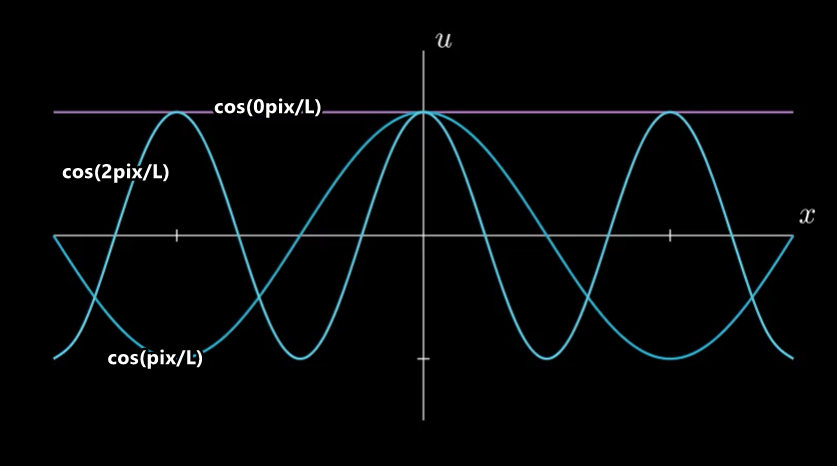
\includegraphics[height=5cm]{Fourier Basis Functions}
  \end{center}

  What happens if you use a Fourier Series on a discontinuous function?
  \begin{align}
    f(x) & =
    \begin{cases}
      1 & x \in (-4, 6)\\
      0 & x \in [-10, -4] \bigcup [6, 10]
    \end{cases}
  \end{align}

  \begin{center}
    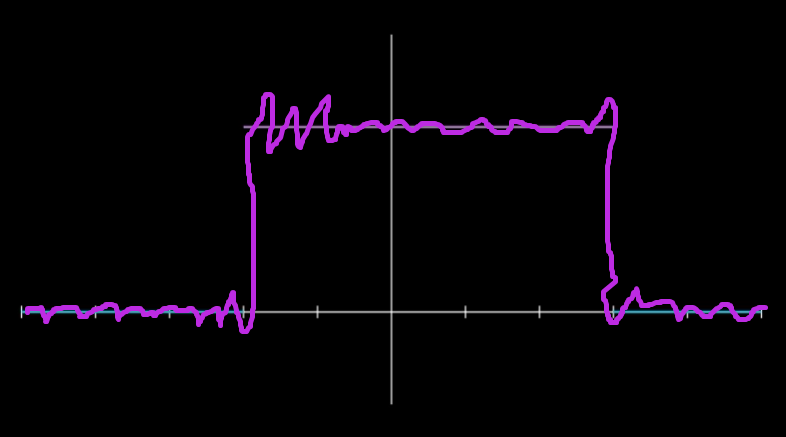
\includegraphics[height=5cm]{Fourier Finite Fourier Series}
  \end{center}

  The Oscillations around the discontinuities are called Gibbs phenomenon. As $M$ increases, the oscillation's amplitude does not change. However, the oscillations do get progressively closer to the discontinuities.

  \begin{center}
    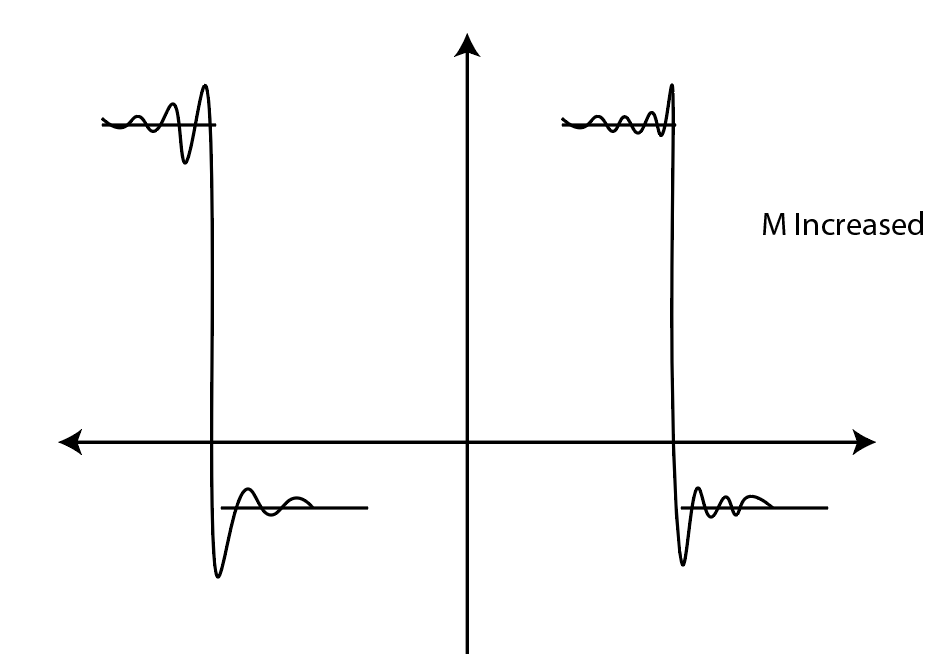
\includegraphics[height=5cm]{Fourier M}
  \end{center}

  If $M = \infty$, then we have:
  \begin{align}
    \text{Fourier Series } =
    \begin{cases}
      f(x) & = \text{ if $x$ is a point of continuity }\\
      \lim_{c \to 0^+} \frac{f(x + c) + f(x - c)}{2} & \text{ if x is a point of discontinuity}
    \end{cases}
  \end{align}

  \begin{center}
    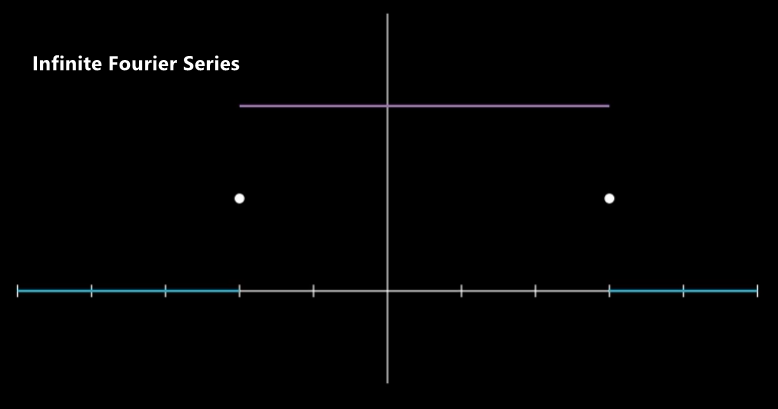
\includegraphics[height=5cm]{Fourier Infinite Fourier Series}
  \end{center}

  \topic{Orthogonality}\\
  Recall: The vectors
  \begin{align}
    u =
    \begin{bmatrix}
      u_1\\
      u_2\\
      \vdots\\
      u_n
    \end{bmatrix}
    \qquad \text{and} \qquad
    v =
    \begin{bmatrix}
      v_1\\
      v_2\\
      \vdots\\
      v_n
    \end{bmatrix}
  \end{align}

  are orthogonal if the dot product is zero.

  \begin{align}
    u \circ v & = \sum^n_{i = 1} u_i v_i = 0
  \end{align}

  We want to generalize this to function $x \in [-L, L]$.

  \dfn Two functions $f(x)$ and $g(x)$ are orthogonal on $[a, b]$ if

  \begin{align}
    \int^b_a f(x)g(x) \dx & = 0
  \end{align}

  \thm All basis functions in the Fourier Series are mutually orthogonal

  \begin{align}
    \int^L_{-L} \sin\Big(\frac{m \pi x}{L}\Big) \FS \dx & = 0 \quad n \neq m\\
    \int^L_{-L} \cos\Big(\frac{m \pi x}{L}\Big) \FC \dx & = 0 \quad n \neq m
  \end{align}
  What happens if $m = n$?
  \begin{align}
    \int^L_{-L} \sin^2\Big( \frac{m \pi x}{L} \Big) \dx
  \end{align}
  Here, we want to use the double angle formula: $\cos(2\theta) = 1 - 2\sin^2 \theta$.
  \begin{align}
    \int^L_{-L} \sin^2\Big( \frac{m \pi x}{L} \Big) \dx & =
    \frac{1}{2} \int^L_{-L} 1 - \cos\Big(\frac{2 m \pi x}{L}\Big) \dx\\ & =
    \frac{1}{2} \Big[ x - \frac{L}{2 m \pi}\sin\Big(\frac{2 m \pi x}{L}\Big)\Big]^L_{-L}\\ & =
    \frac{1}{2} \Big[L - \frac{L}{2 m \pi} \sin(2 m \pi) - \Big(-L - \frac{2}{2 m \pi} \sin(-2 m \pi)\Big)\Big]\\ & =
    L
  \end{align}

  \subsection*{January 28, 2022}
  Similarly,
  \begin{align}
    \int^L_{-L} \cos^2 (\frac{n\pi x}{L}) \dx & = L
  \end{align}
  If $n = 0$,
  \begin{align}
    \int^L_{-L} 1 \dx & = 2L
  \end{align}

  \note You cannot differentiate the Fourier Series term-by-term $f'(x)$ like you can with Taylor series.

  Let's show $\cos(\frac{n \pi x}{L})$ and $\sin(\frac{m \pi x}{L})$ are orthogonal on $[-L, L]$.
  \begin{align}
    \int^L_{-L} \sin\Big(\frac{m \pi x}{L}\Big) \FC \dx & = \frac{1}{2} \int^L_{-L} \sin\Big( \frac{(m + n) \pi x}{L} \Big) + \sin\Big( \frac{(m - n) \pi x}{L} \Big) \dx\\
    & = - \frac{1}{2} \Big[ \frac{L}{(m + n) \pi} \cos\Big(\frac{(m + n) \pi x}{L} \Big) + \frac{L}{(m - n)\pi} \cos\Big( \frac{(m - n) \pi x}{L} \Big) \Big]^L_{-L}
  \end{align}
  Here, we expand our difference and notice we have even and odd functions.

  In general, the coefficients are:
  \begin{align}
    a_n & = \frac{1}{L} \int^L_{-L} f(x) \FS \dx\\
    b_n & = \frac{1}{L} \int^L_{-L} f(x) \FC \dx\\
    b_0 & = \frac{1}{2L} \int^L_{-L} f(x) \dx
  \end{align}

  \Ex $f(x) = x, \quad x \in [-3, 3]$.

  Find the Fourier Series for $f$.

  \begin{align}
    a_n & = \frac{1}{3} \int^3_{-3} x \FS \dx
  \end{align}

  Here, we want to integrate by parts:
  \begin{center}
    \begin{tabular}{c|c}
      $x$ & $\FS$\\
      \hline
      $1$ & $- \frac{3}{n \pi} \FC$\\
      \hline
      $0$ & $- \frac{9}{n^2 \pi^2} \FS$
    \end{tabular}
    \note $L = 3$.
  \end{center}

  \begin{align}
    & = \frac{1}{3} \Big[ -\frac{3 x}{n \pi} \cos\Big( \frac{n \pi x}{3} \Big) \Big]^3_{-3} + \Big[ \Big( \frac{3}{n \pi} \Big)^2 \sin\Big( \frac{n \pi x}{3} \Big)\Big]^3_{-3}\\
    & = \frac{1}{3} \Bigg[ -\frac{9}{n \pi} \cos(n \pi) + \frac{9}{n^2 \pi^2}
    \sin(n \pi) -
    \Big( +\frac{9}{n \pi} \cos(-n \pi) + \frac{9}{n^2 \pi^2} \sin(-n \pi) \Big)\Bigg]\\
    & = -\frac{6}{n \pi} \cos(n \pi)
  \end{align}

\newpage
\subsection*{January 31, 2022}
The Fourier Series is not valid at $x = \pm 3$ since it is not continuous at $\pm 3$.

Let's say $f(x)$ is odd, then $\displaystyle f(x) = \sum^\infty_{n = 1} a_n \FS$

Let's say $f(x)$ is even, then $\displaystyle f(x) = \sum^\infty_{n = 1} b_n \FC$

If we are only interested in the behavior of $f(x)$ on $[0, L$, then we can either use a Fourier Sine Series $\displaystyle f(x) = \sum^\infty_{n = 1} a_n \FS$ or a Fourier series $f(x) = \sum^\infty_{n = 0} b_n \FC$.

\topic{Solving the Heat Equation}

\begin{align}
  u_t & = \alpha^2 u_{xx}
\end{align}
\begin{center}
  0 o============o L
  $u(x, t) : $ temp
\end{center}

Initial condition:
\begin{align}
  u(x, 0) = f(x)
\end{align}
Boundary conditions
\begin{align}
  u(0, t) = u(L, t) = 0
\end{align}
\begin{center}
  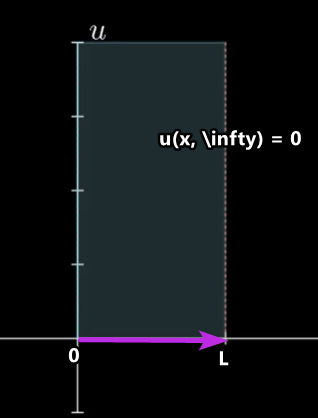
\includegraphics{FourierReflection}
\end{center}
So, whatever we get, we better have $\displaystyle \lim_{t \to \infty} u(x, t) = 0$. The method of reflection? relies on two things:
\begin{enumerate}
  \item Fourier Series
  \item Linearity
\end{enumerate}
\underline{Method}
\begin{enumerate}
  \item Try a solution of the form
  \begin{align}
    u(x, t) = X(x)T(t) \leftarrow \text{ Assume the solution is separable}
  \end{align}
  Boundary Conditions:
  Here, we conclude $X(0)$ is $0$ because we want $T(t)$ to change as $t$ changes.
  \begin{align}
    u(0, t) = 0 & \Rightarrow X(0)T(t) = 0 \Rightarrow X(0) = 0\\
    u(L, t) = 0 & \Rightarrow X(L)T(t) = 0 \Rightarrow X(L) = 0\\
    U_t = \alpha^2 u_{xx} & \Rightarrow X(x)T^\prime(t) = \alpha^2 X^{\prime\prime}(x) T(t)
  \end{align}
  Here, we divide by $X, T, \alpha^2$.
  \begin{align}
    \Rightarrow \frac{T^\prime(t)}{\alpha^2T(t)} & = \frac{X^{\prime\prime}}{X(x)} = -\lambda
  \end{align}
  Here, $\lambda$ is a constant.
  \item
  \begin{align}
    \frac{X^{\prime\prime}}{X(x)} & = -\lambda\\
    X^{\prime\prime}(x) & = -\lambda X(x)
  \end{align}
  Here, we know $(x) = X(L) = 0$. We call every $(\lambda, X(x))$ pair that satisfies this equation an eigenvalue/eigenfunction pair for the differential equation.

  Assume $\lambda > 0$
  \begin{align}
    X^{\prime\prime} & = -\lambda x\\
    x(0) & = x(L) = 0\\
    & \Rightarrow X(x) = A \cos(\sqrt{\lambda} x) + B\sin(\sqrt{\lambda} x)\\
    & \Rightarrow A \cos 0 + B \sin 0 = 0\\
    & \Rightarrow A = 0\\
    & \Rightarrow X(x) = B \sin(\sqrt \lambda x)\\
    X(L) = 0 & \Rightarrow B \sin(\sqrt \lambda L) = 0\\
    & \Rightarrow \sin(\sqrt \lambda L) = 0\\
    & \Rightarrow \sqrt \lambda L = n \pi, n \in \Z^+\\
    & \Rightarrow \lambda_n = \Big( \frac{n \pi}{L} \Big)^2\\
    & \Rightarrow_n(x) = \FS
  \end{align}
\end{enumerate}

\subsection*{February 2, 2022}
\begin{align}
  u(x, t) & = X(x)T(t)\\
  \frac{X^{\prime\prime}}{x} & = \frac{T^\prime}{\alpha^2 T} = - \lambda\\
  \lambda_n & = \left( \frac{n \pi}{L} \right)^2\\
  X_n(x) & = \FS
\end{align}
Here, we have a bsis function for Fourier Sine Series.
\begin{enumerate}
  \setcounter{enumi}{2}
  \item Solve for $T$
  \begin{align}
    \frac{T^\prime}{\alpha^2 T} & = - \lambda\\
    T^\prime & = -\alpha^2 \lambda T\\
    T^\prime_n & = - \alpha^2 \lambda_n T_n\\
    & = -\alpha^2 \left( \frac{n \pi}{L} \right)^2 T
  \end{align}
  If we have something like $y^\prime = ky$, we know that this derives from $y = e^{kx}$.
  \begin{align}
    T_n(t) & = e^{-\alpha^2 \left( \frac{n \pi}{L} \right)^2 T}
  \end{align}
  \item Combine for $u_n$
  \begin{align}
    u_n(x, t) & = X_n(x)T_n(t)\\
    & = \FS e^{-\alpha^2 \left( \frac{n \pi}{L} \right)^2 T}
  \end{align}
  Each one of the $n's$ will yield a different $u$. We also know that $n \in \N$. We can take as many $u'$s and add them all together. We find our $u_n'$s and use it to find $u$.

  By linearity,
  \begin{align}
    u(x, t) & = \sum^\infty_{n = 1} A_n\\
    & = \sum^\infty_{n = 1} A_n \FS e^{-\alpha^2 \left( \frac{n \pi}{L} \right)^2 T}
  \end{align}

  \item Satisfy the initial condition
  \begin{align}
    u(x, 0) & = f(x)\\
    u(x, 0) & = \sum^\infty_{n = 1} A_n \FS = f(x)
  \end{align}
  Line 113) is considered the Fourier Sine Series.

  The $A_n'$s are the coefficients of the Fourier Sine Series of $f(x)$.
  \begin{align}
    A_n & = \frac{1}{L} \int^L_{-L} f(x) \FS dx\\
    & = \frac{2}{L} \int^L_0 f(x) \FS dx
  \end{align}
\end{enumerate}

\ex Solve with the following conditions:
\begin{enumerate}
  \item $u_t = 4u_{xx}$
  \item $u(0, t) = u(3, t) = 0$
  \item $u(x, 0) = 5 \sin \left( \frac{2 \pi x}{3} \right) - 7 \sin(4 \pi x)$
\end{enumerate}
Now, let us perform the five steps to solve our equation:
\begin{enumerate}
  \item Assume $u(x, t) = X(x)T(t)$\\
  Boundary Conditions :
  \begin{itemize}
    \item $u(0, t) = 0$, then $X(0)T(t) = 0$. Here either $X(0)$ or $T(t)$ is $0$, and we want $X(0) = 0$ here.
    \item $(3, t) = 0$, then $X(3)T(t) = 0$, following the same logic, we have $X(3) = 0$.
  \end{itemize}
  \begin{align}
    u_t & = 4u_{xx}\\
    XT^\prime & = 4X^{\prime\prime}T\\
    \frac{T^\prime}{4T} & = \frac{X^{\prime\prime}}{X} = -\lambda
  \end{align}
  \item Now, since we know more information regarding $X$, let us solve for $X$.
  \begin{align}
    \frac{X^{\prime\prime}}{X} & = -\lambda\\
    X^{\prime\prime} & = -\lambda X, \quad X(0) = X(3) = 0
  \end{align}
  Let us assume $\lambda > 0$. Here, we want an $X^{\prime\prime}$ where deriving twice gives us $-X$. Assume $\lambda > 0$
  \begin{align}
    X & = A\sin(\sqrt \lambda x) + B \cos(\sqrt \lambda x)
  \end{align}
  Set $X(0) = 0$
  \begin{align}
    X & = A
  \end{align}
  Now, let us find $X(3) = 0$:
  \begin{align}
    0 & = A\sin(\sqrt \lambda 3)\\
    \sqrt \lambda 3 & = n \pi\\
    \lambda_n & = \left( \frac{n \pi}{3} \right)^2\\
    X_n(x) & = \sin \left(\frac{n \pi x}{3} \right)
  \end{align}
  \item Now, let us find $T$.
  \begin{align}
    \frac{T^\prime}{4T} & = -\lambda\\
    T^\prime_n & = -4 \left( \frac{n \pi}{3} \right)^2 T_n\\
    T_n(t) & = e^{-4 \left( \frac{n^2 \pi^2}{9} \right)t}
  \end{align}
  \item Combine to find $u_n$ and $u$
  \begin{align}
    u_n(x, t) & = X_n(x)T_n(t)\\
    & = \sin\left( \frac{n \pi x}{3} \right) e^{-4 \left( \frac{n^2 \pi^2}{9} \right)t}
  \end{align}
  By linearity,
  \begin{align}
    u(x, t) & = \sum^\infty_{n = 1} A_n \sin\left( \frac{n \pi x}{3} \right) e^{-4 \left( \frac{n^2 \pi^2}{9} \right)t}
  \end{align}
  \item Use the initial conditions to find $A_n'$s
  \begin{align}
    u(x, 0) & = 5\sin(\frac{2 \pi x}{3}) - \sin(4 \pi x)\\
    u(x, 0) & = \sum^\infty_{n = 1} A_n \sin\left( \frac{n \pi x}{3} \right)\\
    A_n & = \frac{2}{3} \int^3_0 5 \left[\sin\left( \frac{2 \pi x}{3} \right) - 7 \sin(4 \pi x) \right] \sin(\frac{n \pi x}{3}) \dx
  \end{align}
  Lets look at our initial condition on line 133). The first one is $n =2$, so $A_2 = 5$. In addition, the second term is at $A_12 = -7$. Therefore, we have $A_n = 0 \forall n$ except $n = 2, 12$.

  Now, let us look at our linearity equation.
  \begin{align}
    u(x, t) & = 5 \sin\left( \frac{2 \pi x}{3} \right) e^{-\frac{16 \pi^2}{9} t} - 7 \sin\left( 4 \pi x \right) e^{-64 \pi^2 t}
  \end{align}
  Here, this is our final solution.

  \topic{Laplace's Equation}
  1-D : $u_{xx} = 0 \Rightarrow u = ax + b$

  If $u(0) = u(L) = 0$, then that would force our function to be $u = 0$. This is the steady state solution. If our function is in the form of $ax + b$, then $u = 0$ is the only solution for the function to hit $0$ twice in this fashion.

  2-D: $\Delta u = 0 \Rightarrow u_{xx} + u_{yy} = 0$

  \begin{center}
    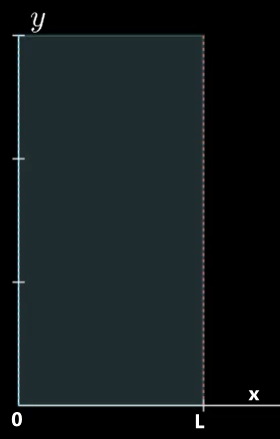
\includegraphics{Laplaces}
  \end{center}

  We have two types of boundary conditions:
  \begin{enumerate}
    \item Specify $u$ on the perimeter
    \begin{itemize}
      \item $u(0, y) = 0$
      \item $u(L, y) = 0$
      \item $u(x, 0) = 0$
      \item $u(x, M) = f(x)$
    \end{itemize}
    \item Nuemann conditions : Specify the direction derivative in the normal direction on the boundary.
    \begin{itemize}
      \item $u_x(0, y) = 0$
      \item $u_x(L, y) = 0$
      \item $u_y(x, 0) = 0$
      \item $u_y(x, M) = \twiddle{f}(x)$
      \item $u(0, 0)\  = T$
    \end{itemize}
    This is if we know the heat flux $\vec q \cdot \vec n$ on the boundary.
  \end{enumerate}
\end{enumerate}
\newpage
\subsection*{February 4, 2022}
\topic{Solving Laplace's Equation}
\begin{center}
  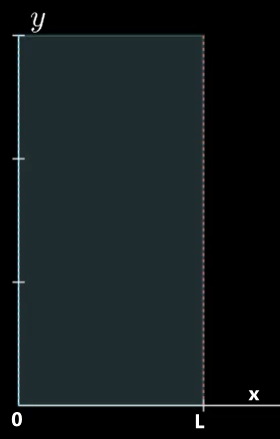
\includegraphics{Laplaces}

  $u_{xx} + u_{yy} = 0$
\end{center}
\begin{itemize}
  \item $u_x(0, y) = 0$
  \item $u_x(L, y) = 0$
  \item $u(x, 0) = 0$
  \item $u(x, M) = f(x)$
\end{itemize}
\begin{enumerate}
  \item Assume $u(x, y) = X(x)Y(y)$

  \underline{Boundary Conditions}
  \begin{align}
    u(x, y) & = X(x) Y(y)\\
    & \Rightarrow X^\prime(x)Y(y)
  \end{align}
  Now, let us write our boundary condition:
  \begin{align}
    U_x(0, y) & = 0\\
    & \Rightarrow X^\prime(0)Y(y) = 0\\
    & \Rightarrow X^\prime(0) = 0
  \end{align}
  Now, let us find the next item,
  \begin{align}
    u_x(L, y) & = 0\\
    & \Rightarrow X^\prime(L)Y(y) = 0\\
    & \Rightarrow X^\prime(L) = 0
  \end{align}
  Now, the next two items do not have a derivative:
  \begin{align}
    u(x, 0) & = 0\\
    & \Rightarrow X(x)Y(0) = 0\\
    & \Rightarrow Y(0) = 0
  \end{align}
  Now, let us write:
  \begin{align}
    u_{xx} + u_{yy} & = 0\\
    & \Rightarrow X^{\prime\prime}Y + XY^{\prime\prime} = 0\\
    & \Rightarrow X^{\prime\prime}Y = - XY^{\prime\prime}\\
    & \Rightarrow \frac{X^{\prime\prime}}{X} = - \frac{Y^{\prime\prime}}{Y} = -\lambda
  \end{align}

  \item Solve for $X$ (Note: We solve for $X$ first here, since we have more information about $X$).
  \begin{align}
    \frac{X^{\prime\prime}}{X} & = - \lambda\\
    \Rightarrow X^{\prime\prime} & = - \lambda X, \quad X^\prime(0) = X^\prime(L) = 0\\
    \lambda > 0 \Rightarrow x(x) & = A \sin(\sqrt \lambda x) + B \cos(\sqrt \lambda x)\\
    \Rightarrow X^\prime(x) & = A \sqrt \lambda \cos(\sqrt \lambda x) - B \sqrt \lambda \sin(\sqrt \lambda x)\\
    X^\prime(0) = 0 \Rightarrow A \sqrt \lambda & = 0
  \end{align}
Now, if we rewrite out equation, we have:
\begin{align}
  X(x) & = B \cos(\sqrt \lambda x)
\end{align}
Next, we want to find $X^\prime(L) = 0$:
\begin{align}
  0 & = - B \sqrt \lambda \sin(\sqrt \lambda L)\\
  \sqrt \lambda L & = n \pi\\
  \lambda_n & = \left(\frac{n \pi}{L}\right)^2\\
  \Rightarrow X_n(x) & = \FC
\end{align}
If $\lambda = 0$
\begin{align}
  \frac{X^{\prime\prime}_0}{X_0} & \Rightarrow X^{\prime\prime}_0 = 0\\
  & \Rightarrow X_0(x) = Ax + B\\
  & \Rightarrow X^\prime_0(x) = A\\
  & \Rightarrow X^\prime_0(0) = 0\\
  & \Rightarrow A = 0\\
  & \Rightarrow X^\prime_0(L) = 0\\
  & \Rightarrow A = 0
\end{align}
Neither conditions tell us more information about $B$,
\begin{align}
  \Rightarrow X_0(x) = B_0
\end{align}
\item Now, we want to solve for $Y$: $- \frac{Y^{\prime\prime}}{Y} = -\lambda$
\begin{align}
  Y^{\prime\prime} & = \lambda y\\
  Y^{\prime\prime} & = \left( \frac{n \pi}{L} \right)^2 Y_n, \quad Y_n(0) = 0\\
  Y_n(y) & = Ce^{\frac{n \pi}{L}y} + De^{- \frac{n \pi}{L}}y\\
  Y_n(0) = 0 & \Rightarrow C + D = 0
\end{align}
Here, we do not have an additional condition that could help use solve this equality. Let us consider the hyperbolic sin and cos:
\begin{align}
  \sinh(x) & = \frac{e^x - e^{-x}}{2}\\
  \cosh(x) & = \frac{e^x + e^{-x}}{2}
\end{align}
Instead of writing $Y$ in the same fashion we solved for $X$, we use the hyperbolic $\sinh$ and $cosh$
\begin{align}
  Y_n(y) & = C \sinh \left(\frac{n \pi y}{L} \right) + D \cosh \left( \frac{n \pi y}{L} \right)\\
  Y_n(0) = 0 & \Rightarrow D = 0\\
  Y_n(y) & = \sinh \left( \frac{n \pi y}{L} \right)
\end{align}
Now, let us write:
\begin{align}
  \frac{Y^{\prime\prime}_0}{Y_0} = \lambda_0 &\\
  & \Rightarrow Y^{\prime\prime}_0 = 0\\
  & \Rightarrow Y_0 = Cy + D\\
  & \Rightarrow Y_0(0) = 0\\
  & \Rightarrow D = 0\\
  & \Rightarrow Y_0(y) = C_0 y
\end{align}
\item Combine to find $u_n$ and $u$:
\begin{align}
  u_n(x, y) = X_n(x)Y_n(y) & =
  \begin{cases}
    \FC \sinh \left( \frac{n \pi y}{L} \right) & n \geq 1\\
    B_0C_0y & n = 0
  \end{cases}
\end{align}
By linearity,
\begin{align}
  u(x, y) & = \twiddle{B}_0 y + \sum^\infty_{n = 1} B_n \FC \sinh \left( \frac{n \pi y}{L} \right)
\end{align}
\item Here, use the final boundary condition to find the coefficients.
\begin{align}
  u(x, M) & = f(x)\\
  u(x, M) & = \twiddle{B}_0 M + \sum^\infty_{n = 1} B_n \FC \sinh\left( \frac{n \pi M}{L} \right)
\end{align}
This is our Fourier Cosine Series for $f(x)$. Here, we can say a few things about this equation,
\begin{itemize}
  \item $b_0 = \twiddle B_0 M$
  \item $b_n = B_n \sinh\left( \frac{n \pi M}{L} \right)$
\end{itemize}
\begin{align}
  \twiddle B_0 M & = \frac{2}{2L} \int^L_0 f(x) \dx\\
  \twiddle B_0 & = \frac{1}{ML} \int^L_0 f(x) \dx
\end{align}
Next, let us find:
\begin{align}
  B_n \sinh\left( \frac{n \pi M}{L} \right) & = \frac{2}{L} \int^L_0 f(x) \FC \dx\\
  & = \frac{2}{L \sinh\left( \frac{n \pi M}{L} \right)} \int^L_0 f(x) \FC \dx
\end{align}
\end{enumerate}
\ex Solve $\Delta u = 0$
\begin{itemize}
  \item $(x, y) = 0$
  \item $(2, y) = 0$
  \item $(x, 0) = 0$
  \item $(x, 3) = 4 \sin (5x)$
\end{itemize}
\begin{enumerate}
  \item Assume $u(x, y) = X(x)Y(y)$

  Here, let us look at our boundary conditions:
  \begin{align}
    u(0, y) & = 0\\
    X(0)Y(y) & = 0\\
    X(0) = 0
  \end{align}

  Here, let us look at our next boundary conditions:
  \begin{align}
    u(2, y) & = 0\\
    X(2)Y(y) & = 0\\
    X(2) = 0
  \end{align}

  Here, let us look at our next boundary conditions:
  \begin{align}
    u(x, 0) & = 0\\
    X(x)Y(0) & = 0\\
    Y(x) = 0
  \end{align}

  Now, we can write:
  \begin{align}
    u_{xx} + u_{yy} & = 0\\
    X^{\prime\prime}Y + XY^{\prime\prime} & = 0\\
    \frac{X^{\prime\prime}}{X} & = -\frac{Y^{\prime\prime}}{Y} = - \lambda
  \end{align}
  \item Now, let us solve for $x$:
  \begin{align}
    \frac{X^{\prime\prime}}{X} & = -\lambda\\
    X^{\prime\prime} & = - \lambda X, \quad X(0) = X(2) = 0\\
    \lambda > 0 \Rightarrow X(x) & = A \sin(\sqrt \lambda x) + B \cos(\sqrt \lambda x)\\
    X(0) & = B = 0\\
    X(2) & = A \sin(\sqrt \lambda 2) = 0\\
    & = \lambda 2 = n \pi\\
    & = \lambda_n = \left( \frac{n \pi}{2} \right)^2\\
    & = X_n(x) =  \sin(\frac{n \pi x}{2})
  \end{align}
  \item Let us solve for $y$:
  \begin{align}
    \frac{Y^{\prime\prime}_n}{Y_n} & = \lambda_n\\
    Y^{\prime\prime}_n & = \left(\frac{n \pi}{2}\right)^2 Y_n, \quad Y_n(0) = 0\\
    Y_n(y) & = C \sinh \left( \frac{n \pi y}{2} \right) + D \cosh \left( \frac{n \pi y}{2} \right)\\
    & = Y_n(0) = 0 \Rightarrow D = 0\\
    Y_n(y) & = \sinh \left( \frac{n \pi y}{2} \right)
  \end{align}
  We are picking a constant for this last term later, so we can drop $C$.
\end{enumerate}
Here, let us write out our equation for the following function,

\subsection*{February 7, 2022}
\begin{itemize}
  \item $\Delta u = 0$
  \item $u(0, y) = 0$
  \item $u(2, y) = 0$
  \item $u(x, 0) = 0$
  \item $u(x, 3) = 4$
  \item $\lambda_n = \left(\frac{n \pi}{2}\right)^2$
  \item $X_n(x) = \sin\left(\frac{n \pi x}{2}\right)$
  \item $Y_n(x) = \sinh\left(\frac{n \pi y}{2}\right)$
\end{itemize}
\begin{enumerate}
  \setcounter{enumi}{3}
  \item Combine to find $u_n$ and $u$
  \begin{align}
    u_n(x, y) = \sin\left( \frac{n \pi x}{2} \right)\sinh\left(\frac{n\pi y}{2} \right)
  \end{align}
  By linearity,
  \begin{align}
    u(x, y) = \sum^\infty_{n = 1} A_n \sin\left( \frac{n \pi x}{2} \right) \sinh\left( \frac{n \pi y}{2} \right)
  \end{align}
  \item Find coefficients using last boundary conditions
  \begin{align}
    u(x, y) & = 4 \sin(5 \pi x)\\
    u(x, y) & = \sum^\infty_{n = 1} A_n \sin\left(\frac{n \pi x}{2} \right) \sinh\left(\frac{n \pi 3}{2} \right)\\
    & = 4\sin(5 \pi x)
  \end{align}
  Recall, the coefficient of the Fourier Sine Series is anything but $\sin$. Notice our last line with discrete number, our coeficient must equal $4$ and our $n$ is 10, therefore, we write:
  \begin{align}
    A_{10} & \sinh\left( \frac{10 \pi 3}{2} \right) = 4\\
    \Rightarrow A_10 & \frac{4}{\sinh(15 \pi)}
  \end{align}
\end{enumerate}

\topic{The Wave Equation}
\begin{align}
  u_{tt} & = c^2 u_{xx}
\end{align}
Boundary conditions:
\begin{align}
  u(0, t) & = u(L, t) = 0
\end{align}
Initial Conditions:
\begin{align}
  u(x, 0) & = f(x)\\
  u_t(x, 0) & = g(x)
\end{align}
Here, $g \in C^2$, $g(0) = g(L)$.
\begin{enumerate}
  \item Assume separable:

  \begin{align}
    u(x, t)
  \end{align}

  Boundary conditions:
  \begin{align}
    u(0, t) = 0 & \Rightarrow X(0)T(t) = 0 \Rightarrow X(0) = 0\\
    u(L, t) = 0 & \Rightarrow X(L)T(t) = 0 \Rightarrow X(L) = 0
  \end{align}
  Now, let us rewrite our variables:
  \begin{align}
    u_{tt} & = c^2u_{xx}\\
    XT^{\prime\prime} & = c^2 X^{\prime\prime}T\\
    \frac{T^{\prime\prime}}{c^2 T} & = \frac{X^{\prime\prime}}{X} = -\lambda
  \end{align}
  \item Solve for $X$:
  \begin{align}
    \frac{X^{\prime\prime}}{X} & = -\lambda\\
    X^{\prime\prime} & = -\lambda x\\
    X(0) & = X(L) = 0
  \end{align}
  Here, let us write our general equation:
  \begin{align}
    X(x) & = A\sin(\sqrt \lambda x) + B \cos (\sqrt \lambda x)\\
    X(0) & = 0 \Rightarrow B = 0\\
    X(L) & = A \sin(\sqrt \lambda L) = 0\\
    & = \sqrt \lambda L = n \pi
  \end{align}
  \item Solve for $T$:
  \begin{align}
    \frac{T^{\prime\prime}}{c^2 T_n} & = - \lambda_n\\
    T^{\prime\prime}_n & = -c^2 \left( \frac{n \pi}{L} \right)^2 T_n\\
    T_n(t) & = C_n \sin \left( \frac{c n \pi t}{L} \right) + D_n \cos \left( \frac{c n \pi t}{L} \right)
  \end{align}
  \item Combine to find $u_n$ and $u$
  \begin{align}
    u_n(x, t) & = \FS \left[ C_n \sin\left(\frac{ c n \pi z}{L} \right) + D_n \cos \left( \frac{c n \pi z}{L} \right) \right]\\
    u(x, t) & = \sum^\infty_{n = 1} c_n \FS \sin \left( \frac{c n \pi z}{L}\right) + D_n \FS \cos \left( \frac{c n \pi z}{L} \right)
  \end{align}
  \item Find coefficients using Inidial Conditions
  \begin{align}
    u(x, 0) & = f(x)\\
    & = \sum^\infty_{n = 1} D_n \FS = f(x)\\
    D_n & = \frac{2}{L} \int^L_0 f(x) \FS \dx\\
    u_t(x, 0) & = g(x)\\
    u_t(x, t)
  \end{align}
  Here, we took the $t$ partial from line 246.
  \begin{align}
    u_t(x, t) & = \sum^\infty_{n = 1} C_n \FS \frac{c n \pi}{L} \cos \left(\frac{c n \pi t}{L}\right) - D_n \FS \frac{c n \pi}{L} \sin\left( \frac{c n \pi t}{L} \right)\\
    u_t(x, 0) & = \sum^\infty_{n = 1} C_n \FS \frac{c n \pi}{L} = g(x)
  \end{align}
  Here, the non-sin terms are the coefficients of the Fourier Sine Series.
  \begin{align}
    C_n \frac{c n \pi}{L} & = \frac{2}{L} \int^L_0 g(x) \FS \dx\\
    C_n & = \frac{2}{c n \pi} \int^L_0 g(x) \FS \dx
  \end{align}
\end{enumerate}
\thm You can differentiate a Fourier Series if it represents a $C^2$ function that is the same as the endpoints.

\ex Solve $u_{tt} = u_{xx}$
\begin{itemize}
  \item $u(0, t)   = 0 $
  \item $u(4, t)   = 0 $
  \item $u(x, 0)   = 2 \sin(3 \pi x) - \frac{1}{5} \sin\left( \frac{7 \pi x}{2} \right)$
  \item $u_t(x, 0) = 0$
\end{itemize}
\begin{enumerate}
  \item Assume separable
  \begin{align}
    u(x, t) = X(x)T(t)
  \end{align}
  Here, we have our boundary conditions,
  \begin{align}
    u(0, t) & = 0 \Rightarrow X(0)T(t) = 0 \Rightarrow X(0) = 0\\
    u(4, t) & = 0 \Rightarrow X(4)T(t) = 0 \Rightarrow X(4) = 0
  \end{align}
  Now, let us separate:
  \begin{align}
    u_{tt} & = u_{xx}\\
    XT^{\prime\prime} & = X^{\prime\prime}T\\
    \frac{T^{\prime\prime}}{T} & = \frac{X^{\prime\prime}}{X} = -\lambda
  \end{align}
  \item Solve for $x$:
  \begin{align}
    \frac{X^{\prime\prime}}{X} & = - \lambda\\
    X^{\prime\prime} & = -\lambda x\\
    X(0) & = X(4) = 0\\
    X(x) & = A \sin(\sqrt \lambda x) + B \cos (\sqrt \lambda x)\\
    X(0) & = B = 0\\
    X(4) & = A \sin(\sqrt \lambda 4) = 0\\
    & = \sqrt \lambda 4 = n \pi\\
    & = \lambda_n = \left( \frac{n \pi}{4} \right)^2\\
    & = X_n(x) = \sin\left( \frac{n \pi x}{4}\right)
  \end{align}
  \item Solve for $T$:
  \begin{align}
    \frac{T^{\prime\prime}_n}{T_n} & = - \lambda_n\\
    T^{\prime\prime}_n & = - \left( \frac{n \pi}{4} \right)^2 T_n
  \end{align}
  Here, we have the negative sign, therefore we use sine and cosine:
  \begin{align}
    T_n(t) & = C_n \sin \left( \frac{n \pi t}{4} \right)
  \end{align}
  \item Combine to get $u_n$ and $u$
  \begin{align}
    u_n(x, t) & = \sin\left(\frac{n \pi x}{4}\right) + D_n \cos \left( \frac{n \pi t}{4} \right)
  \end{align}
  By linearity,
  \begin{align}
    u(x, t) & = \sum^\infty_{n = 1} C_n \sin\left( \frac{n \pi x}{4} \right) + D_n \sin\left( \frac{n \pi t}{4} \right) \cos\left( \frac{n \pi t}{4} \right)
  \end{align}
  \item Use the initial conditions to find the coefficients
  \begin{align}
    u(x, 0) & = 2 \sin (3 \pi x) - \frac{1}{5} \sin \left( \frac{ 7 \pi x}{2} \right)\\
    u(x, 0) & = \sum^\infty_{n = 1} D_n \sin\left( \frac{n \pi x}{4} \right)\\
    & D_{12} = 2, D_{14} = -\frac{1}{5}, D_n = 0 \ \forall n, n \neq 12, 14\\
    u_t(x, t) & = \sum^\infty_{n = 1} C_n \sin\left( \frac{n \pi x}{4} \right) \frac{n \pi}{4} \cos\left( \frac{n \pi t}{4} \right) - D_n \sin\left( \frac{n \pi x}{4} \right) \frac{n \pi}{4} \sin\left( \frac{n \pi t}{4} \right)\\
    u_t(x, 0) & = \sum^\infty_{n = 1} C_n \sin\left( \frac{n \pi x}{4} \right) \frac{n \pi}{4} = g(x) = 0\\
    & C_n = 0 \ \forall n\\
    u(x, t) & = 2 \sin(3 \pi x) \cos(3 \pi t) - \frac{1}{5} \sin\left( \frac{7 \pi x}{2} \right) \cos\left( \frac{7 \pi t}{2} \right)
  \end{align}
\end{enumerate}

\newpage

\subsection*{February 9, 2022}
\topic{More general Boundary Conditions}

Before, we used to deal with boundary conditions where $u$ starts and end at $0$. Now, let us consider boundary conditions where $u$ can start at any number.

% To view different conditions, visit Visual Studio code, credits to @199071614166499328.

The steady state solution is the following:
%
\begin{align}
  \frac{T_2 - T_1}{L} x + T_1
\end{align}

Ideas, we want to try the following: $u(x, t) = w(x, t) + u(x, \infty)$. Note that $\infty$ is the steady state. Here, as time goes to infinity, $w(x, t)$ cancels out. We want to solve for $w$:

We must specify $w$.
%
\begin{align}
  u_t & = \alpha^2 u_{xx}\\
  w_t & = \alpha^2 w_{xx}
\end{align}

We want to find out more about the boundary conditions. We also need the initial conditions to solve this.

\underline{Boundary Conditions}
\begin{itemize}
  \item $u(0, t) = T_1$
  \item $u(L, t) = T_2$
\end{itemize}

Let us consider the first boundary condition.
%
\begin{align}
  w(0, t) + u(0, \infty) & = T_1
\end{align}

Here, we know that for the steady state, $x$ is $T_1$ at $x = 0$. Therefore,
%
\begin{align}
  w(0, t) & = 0
\end{align}

We repeat with our second bullet.
%
\begin{align}
  u(L, t &) = T_2 \Rightarrow\\
  w(L, t) + u(L, \infty) & = T_2\\
  w(L, t) & = 0
\end{align}

\underline{Initial Conditions}
%
\begin{align}
  u(x, 0) & = f(x) \Rightarrow\\
  w(x, 0) + u(x, \infty) & = f(x)\\
  w(x, 0) & = f(x) - u(x, \infty)\\
  w(x, 0) & = f(x) - \left[ \frac{T_2 - T_1}{L} x + T_1 \right]
\end{align}

\ex

Solve $u_t = u_{xx}$, $u(0, t) = 2$, $u(4, t) = 3$, $u(x, 0) = -6 \sin(\pi x) + \frac{x}{4} + 2$.

First, find the steady-state solution:
%
\begin{align}
  u(x, \infty) & = \frac{3 - 2}{4} x + 2\\
  & = \frac{x}{4} + 2
\end{align}

Now, we assume $u(x, t) = w(x, t) + u(x, \infty)$. We can make the following assumption:
%
\begin{align}
  u_t = u_{xx} & \Rightarrow w_t = w_{xx}
\end{align}

\underline{Boundary Conditions}
\begin{align}
  u(0, t) = 2 & \Rightarrow w(0, t) = u(0, t) - u(0, \infty) = 2 - 2 = 0\\
  u(4, t) = 3 & \Rightarrow w(4, t) = u(4, t) - u(4, \infty) = 3 - 3 = 0
\end{align}

Here, we plug in our $x$ into our steady-state solution and get 2, 3.

\underline{Initial Conditions}

\begin{align}
  w(x, 0) & = u(x, 0) - u(x, \infty)\\
  & = -\sin(\pi x) + \frac{x}{4} + 2 - \left(\frac{x}{4} + 2\right)\\
  & = -\sin(\pi x)
\end{align}

Now, solve for $w$:
\begin{enumerate}
  \item Assume $w(x, t) = X(x)T(t)$

  \underline{Boundary Conditions}

  \begin{align}
    w(0, t) = 0 & \Rightarrow X(0)T(t) = 0 \Rightarrow X(0) = 0\\
    w(4, t) = 0 & \Rightarrow X(4)T(t) = 0 \Rightarrow X(4) = 0\\
    w_t & = w_{xx} \Rightarrow XT^\prime & = X^{\prime\prime T} \Rightarrow \frac{T^\prime}{T} = \frac{X^{\prime\prime}}{X} = - \lambda
  \end{align}

  \item Solve for $X$ :
  %
  \begin{align}
    \frac{X^{\prime\prime}}{X} & = - \lambda \Rightarrow\\
    X^{\prime\prime} & = -\lambda X\\
    X(0) & = X(4) = 0
  \end{align}

  Here, let us write our general equation:
  %
  \begin{align}
    X(x) & = A \sin(\sqrt \lambda x) + B \cos(\sqrt \lambda x)\\
    X(0) = 0 & \Rightarrow B = 0\\
    X(4) = 0 & \Rightarrow A \sin(\sqrt \lambda 4) = 0\\
    & \Rightarrow \sqrt \lambda 4 = n \pi\\
    & \Rightarrow \lambda_n = \left(\frac{n \pi}{4} \right)^2\\
    & \Rightarrow X_n(x) = \sin\left( \frac{n \pi x}{4} \right)
  \end{align}

  \item Solve for $T$:
  %
  \begin{align}
    \frac{T^\prime_n}{T_n} & = -\lambda_n\\
    T^\prime_n & = -\left( \frac{n \pi}{4} \right)^2 T_n\\
    T_n(t) & = e^{- \left( \frac{n \pi}{4} \right)^2 t}
  \end{align}

  \item Combine to find $w_n$ and $w$:
  %
  \begin{align}
    w_n(x, t) & = \sin\left(\frac{n \pi x}{4} \right)e^{-\left(\frac{n \pi}{4} \right)^2 t}
  \end{align}

  By linearity,
  %
  \begin{align}
    w(x, t) & = \sum^\infty_{n = 1} A_n \sin\left(\frac{n \pi x}{4} \right)e^{-\left( \frac{n \pi}{4} \right)^2 t}
  \end{align}

  \item Find coefficients using Initial Condition
  %
  \begin{align}
    w(x, 0) & = -\sin(\pi x)\\
    w(x, 0) & = \sum^\infty_{n = 1} A_n \sin\left(\frac{n \pi x}{4}\right)\\
    & = -6 \sin(\pi x)\\
    w(x, t) & = -6 \sin(\pi x) e^{-\pi^2 t}
  \end{align}
  Here, $a_4 = -6$.
  %
  \begin{align}
    u(x, t) & = -6 \sin(\pi x)e^{-\pi^2 t} + \frac{x}{4} + 2
  \end{align}
\end{enumerate}
\topic{Laplace's Equation}
\topic{General Dirichlet Boundary Conditions}
\begin{itemize}
  \item $u(x, 0) = f_1(x)$
  \item $u(x, M) = f_2(x)$
  \item $u(0, y) = f_3(y)$
  \item $u(L, y) = f_4(y)$
\end{itemize}

Write our solution as the following:
\begin{align}
  u(x, y) = u_1(x, y) + u_2(x, y) + u_3(x, y) + u_4(x, y)
\end{align}

% Change this into a 4-multi col
\begin{itemize}
  \item $\Delta u_1 = 0$
  \begin{itemize}
    \item $u_1(x, 0) = f_1(x)$
    \item $u_1(x, M) = 0$
    \item $u_1(0, y) = 0$
    \item $u_1(L, y) = 0$
  \end{itemize}
  \item $\Delta u_1 = 0$
  \begin{itemize}
    \item $u_2(x, 0) = 0$
    \item $u_2(x, M) = f_2(x)$
    \item $u_2(0, y) = 0$
    \item $u_2(L, y) = 0$
  \end{itemize}
  \item $\Delta u_1 = 0$
  \begin{itemize}
    \item $u_3(x, 0) = 0$
    \item $u_3(x, M) = 0$
    \item $u_3(0, y) = f_3(y)$
    \item $u_3(L, y) = 0$
  \end{itemize}
  \item $\Delta u_1 = 0$
  \begin{itemize}
    \item $u_4(x, 0) = 0$
    \item $u_4(x, M) = 0$
    \item $u_4(0, y) = 0$
    \item $u_4(L, y) = f_4(y)$
  \end{itemize}
\end{itemize}

This method works because Laplace's equation is linear.

We have already seen that for $u_2$ :
%
\begin{align}
  u_2(x, y) & = \sum^\infty_{n = 1} B_n \sin\left( \frac{n \pi x}{L} \right) \sinh\left( \frac{n \pi y}{L} \right)\\
  u_2(x, M) & = f_2(x)\\
  & \Rightarrow \sum^\infty_{n = 1} B_n \sin\left ( \frac{n \pi x}{L} \right) \sinh\left( \frac{n \pi M}{L} \right)\\
  & = f(x)
\end{align}

Here, $B_n \sinh\left( \frac{n \pi M}{L}\right)$ is the coefficient for Laplace.
%
\begin{align}
  B_n \sinh \left( \frac{n \pi M}{L} \right) & = \frac{2}{L} \int^L_0 f_2(x) \sin\left(\frac{n \pi x}{L}\right) \dx\\
  B_n & = \frac{2}{L \sinh\left(\frac{n \pi M}{L}\right)} \int^L_0 f_2(x) \sin\left(\frac{n \pi x}{L}\right) \dx
\end{align}

Similarly, for $u_4$,
%
\begin{align}
  u_4(x, y) & = \sum^\infty_{n = 1} D_n \sin\left(\frac{n \pi y}{M}\right)\sinh\left(\frac{n \pi x}{L}\right)\\
  u_4(L, y) & = f_4(y)\\
  & \Rightarrow \sum^\infty_{n = 1} D_n \sin\left(\frac{n \pi y}{M}\right) \sinh\left(\frac{n \pi L}{M}\right)\\
  & = f_4(y)
\end{align}

\bigbreak

\subsection*{February 11, 2022}
Recall we are consider $u = u_1 + u+2 + u_3 + u_4$. Let us write:
%
\begin{align}
  u_4(x, y) & = \sum^\infty_{n = 1} D_n \sin\left( \frac{n \pi y}{M}\right)\sinh\left(\frac{n \pi x}{M}\right)\\
  u_4(L, y) & = f_4(y)\\
  & = \sum^\infty_{n = 1} D_n \sin\left( \frac{n \pi y}{M} \right) \sinh\left( \frac{n \pi L}{M} \right) = f_4(y)
\end{align}

Recall, our coefficient is $D_n$ and the $\sinh$ function.
%
\begin{align}
  D_n \sinh\left( \frac{n \pi L}{M} \right) & =
  \frac{2}{M} \int^M_0 f_4(y) \sin\left( \frac{n \pi y}{M} \right) dy\\
  %
  D_n & = \frac{2}{M \sinh\left( \frac{n \pi L}{M} \right)} \int^M_0 f_4(y) \sin\left( \frac{n \pi y}{M} \right) dy
\end{align}

Let's look at $u_1$:
\begin{itemize}
  \item $\Delta u_1 = 0$
  \item $u_1(x, 0) = f_1(x)$
  \item $u_1(x, M) = 0$
  \item $u_1(0, y) = 0$
  \item $u_1(L, y) = 0$
\end{itemize}

\begin{enumerate}
  \item Here, let us consider $\Delta u_1 = 0$:

  \begin{align}
    \frac{X^{\prime\prime}}{X} & = -\frac{Y^{\prime\prime}}{y} = -\lambda\\
    u_1(x, y) & = X(x)Y(y)
  \end{align}

  Boundary Conditions
  %
  \begin{align}
    u_(x, M) & = 0 \Rightarrow X(x)Y(M) = 0 \Rightarrow Y(M) = 0\\
    u_(0, M) & = 0 \Rightarrow X(0)Y(M) = 0 \Rightarrow X(0) = 0\\
    u_(L, M) & = 0 \Rightarrow X(L)Y(M) = 0 \Rightarrow X(L) = 0\\
  \end{align}

\item $\lambda_n = \left( \frac{n \pi}{L} \right)^2$, $X_n(x) = \sin\left( \frac{n \pi x}{L} \right)$

\item Solve for $y$:
%
\begin{align}
  \frac{Y^{\prime\prime}}{Y_n} & = \lambda_n\\
  Y^{\prime\prime}_n & = \left( \frac{n \pi}{L} \right)^2 Y_n\\
  Y_n(y) & = C\sinh \left( \frac{n \pi y}{L} \right) + D \cosh \left( \frac{n \pi y}{L} \right)
\end{align}

Let us see what we have with $Y(m) = 0$:
%
\begin{align}
  C \sinh \left( \frac{n \pi M}{L} \right) + D \cosh \left( \frac{n \pi M}{L} \right) & = 0
\end{align}

Here, this does not work for us. Let us go back and change our $Y_n(y)$:
%
\begin{align}
  Y_n(y) & = C \sinh \left(\frac{n \pi (M - y)}{L} \right) + D \cosh \left( \frac{n \pi (M - y)}{L} \right)
\end{align}

Now, let us use our $Y$:
%
\begin{align}
  Y_n(M) & = C \sinh \left(\frac{n \pi (M - M)}{L} \right) + D \cosh \left( \frac{n \pi (M - M)}{L} \right)\\
  & = D = 0\\
  Y_n(y) & = \sinh\left( \frac{n \pi (M -y)}{L} \right)
\end{align}

\item Let us combine:
%
\begin{align}
  u_m(x, y) & = \FS \sinh\left( \frac{ n \pi (M - y)}{L} \right)
\end{align}

By linearity
%
\begin{align}
  u_1(x, y) & = \sum^\infty_{n = 1} A_n \FS \sinh\left( \frac{n \pi(M -y)}{L} \right)
\end{align}

\item Find coefficients:
%
\begin{align}
  u_1(x, 0) & = f_1(x)\\
  & = \sum^\infty_{n = 1} A_n \FS \sinh\left( \frac{n \pi M}{L} \right) = f_1(x)
\end{align}

Once more, we have our coefficient with $A_n$ and $\sinh$.
%
\begin{align}
  A_n \sinh \left( \frac{n \pi M}{L} \right) & = \frac{2}{L} \int^L_0 f_1(x) \FS \dx\\
  A_n & = \frac{2}{L \sinh \left( \frac{n \pi M}{L} \right)} \int^L_0 f_1(x) \FS \dx
\end{align}

\topic{Wave Equation}

\begin{center}
  \begin{tabular}{r|c|l}
    t & \# &\\
    & \# & \\
    $u = H_1$ & \# & $u = H_2$\\
    & \# &\\
    \hline
  \end{tabular}\\
  0 \quad L\\
  $u(x, 0) = f(x)$\\
  $u_t(x, 0) = g(x)$
\end{center}

Steady-state:
%
\begin{align}
  u_t & = 0 \Rightarrow u_{tt} = 0 \Rightarrow u_{xx} = 0 \Rightarrow u = \frac{H_2 - H_1}{L} x + H_1
\end{align}

Try a solution of the form : $u(x, t) = w(x, t) + u(x, \infty)$. Therefore, $w(x, t) = u(x, t) - u(x, \infty)$.
%
\begin{align}
  u_{tt} & = c^2 u_{xx} \Rightarrow w_{tt} = c^2 w_{xx}
\end{align}

Boundary conditions:
%
\begin{align}
  w(0, t) & = u(0, t) - u(0, \infty) = H_1 - H_1 = 0\\
  w(L, t) & = u(L, t) - u(L, \infty) = H_2 - H_2 = 0
\end{align}

Initial Conditions
%
\begin{align}
  w(x, 0) & = u(x, 0) - u(x, \infty) = f(X) - \frac{H_2 - H_1}{L} x + H_1\\
  w_t(x, t) & = u_t(x, t) \Rightarrow w_t(x, 0) = u_t(x, 0) = g(x)
\end{align}
\end{enumerate}

\topic{Laplace's Equation in Polar Coordinates}

Let's say we want to solve $\Delta u = 0$ with Dirichlet Boundary Conditions on a disk or annulus.

Problem: $\Delta u = u_{xx} + u_{yy} \leftarrow $ in terms of $x$ and $y$.

We must find it in terms of $r$ and $\theta$.
%
\begin{align}
  u(x, y) \rightarrow u(r, \theta)\\
  x & = r \cos \theta\\
  y & = r \sin \theta\\
  r & = \sqrt{x^2 + y^2}\\
  \theta & = \arctan \frac{y}{x}\\
  \tan \theta & = \frac{y}{x}
\end{align}

We are going to find : $u_x, u_{xx}, u_{yy}$
%
\begin{enumerate}
  \item $u_x$ :
  %
  \begin{align}
    u(x, y) & = u( x(r, \theta), y(r, \theta)) = u(r, \theta) = u(r(x, y), \theta(x, y))
  \end{align}
  Here, we break our chain rule as the following:
  \begin{center}
    $u$\\
    $|$ \quad \quad $|$\\
    $r$ \quad \quad $\theta$\\
    $|$ \quad $|$ \quad $|$ \quad $|$\\
    $x$ \quad $y$ \quad $x$ \quad $y$
  \end{center}

  According to our tree, we have two routes.
  %
  \begin{align}
    \frac{\p u}{\p x} & = \frac{\p u}{\p r} \frac{\p r}{\p x} + \frac{\p u}{\p \theta} \frac{\p \theta}{\p x}\\
    & = u_r \frac{x}{\sqrt{x^2 + y^2}} + u_\theta \frac{- \frac{y}{x^2}}{1 + \left( \frac{y}{x}\right)^2}
  \end{align}

  Note that we know $r$ from line 370. We can rewrite $r$ as $(x^2 + y^2)^{\frac{1}{2}}$.

  Now, let us multiply our equation by $\frac{x^2}{x^2}$.
  %
  \begin{align}
    & = u_r \frac{x}{\sqrt{x^2 + y^2}} + u_\theta \frac{- \frac{y}{x^2}}{1 + \left( \frac{y}{x}\right)^2} \cdot \frac{x^2}{x^2}\\
    & = u_r \frac{r \cos\theta}{r} - u_\theta \frac{r \sin \theta}{r^2}\\
    & = u_r \cos\theta - u_\theta \frac{\sin \theta}{r}
  \end{align}
\end{enumerate}

%

\subsubsection*{February 14, 2021}

Idea: What if we are on a disk?

\begin{align}
  \Delta u  & = 0 \Rightarrow u_{xx} + u_{yy} = 0\\
  u_x       & = u_r \cos \theta u_\theta \frac{\sin \theta}{r}\\
  u_{xx}    & = \\
  & = \frac{\p}{\p x} [u_x]\\
  & = \frac{\p u_x}{\p r} \frac{\p r}{\p x} + \frac{\p u_x}{\p \theta} \frac{\p \theta}{\p x}\\
  & =
  \frac{\p}{\p r}
  \left[u_r \cos \theta -u_\theta \frac{\sin \theta}{r}\right] +
  \frac{\p}{\p \theta}
  \left[ u_r \cos \theta - u_\theta \frac{\sin \theta}{r} \right]
  \left[ - \frac{\sin \theta}{r}\right]\\
  & =
  \left[ u_{rr} \cos \theta - u_{\theta r} \frac{\sin \theta}{r} + u_\theta \frac{\sin \theta}{r^2} \right] \cos \theta +
  \left[ u_{r \theta} \cos \theta - u_r \sin \theta - u_{\theta \theta} \frac{\sin \theta}{r} - u_\theta \frac{\cos \theta}{r} \right]
  \frac{\sin \theta}{r}\\
  & =
  u_{rr} \cos^2 \theta
  - 2 u_{\theta r} \frac{\sin \theta \cos \theta}{r}
  + 2 u_\theta \frac{\sin \theta \cos \theta}{r^2}
  + u_r \frac{\sin^2 \theta}{r} + u_{\theta \theta} \frac{\sin^2 \theta}{r^2}\\
  u_{yy} &
  = u_{rr} \sin^2 \theta
  + 2u_{\theta r} \frac{\sin \theta \cos \theta}{r}
  - 2u_\theta \frac{\sin \theta \cos \theta}{r^2}
  + u_r \frac{\cos^2 \theta}{r}
  + u_{\theta \theta} \frac{\cos^2 \theta}{r^2}\\
  \Delta u & = u_{xx} + u_{yy} \\ &
  = u_{rr}
  + \frac{u_r}{r}
  + \frac{u_{\theta \theta}}{r^2} = 0
\end{align}

\topic{Solving Laplace's Equation in Polar Coordinates}

If we have an open disk, akin to a washer, we have two boundaries: The innter boundary and outer boundary.
%
\begin{enumerate}
  \item Assume $u(r, \theta) = R(r) \Theta(\theta)$
  %
  \begin{align}
    u_{rr} + \frac{u_r}{r} + \frac{u_{\theta\theta}}{r^2} & = 0\\
    R^{\prime\prime}\Theta + \frac{R^\prime \Theta}{r} + \frac{R\Theta^{\prime\prime}}{r^2} & = 0\\
    R^{\prime\prime} \Theta + \frac{R^\prime \Theta}{r} & = - \frac{R \Theta^{\prime\prime}}{r^2}\\
    \frac{r^2}{R^{\prime\prime}}{R} + \frac{r R^\prime}{R} & = - \frac{\Theta^{\prime\prime}}{\Theta} = \lambda
  \end{align}

  \item Solve for $\Theta$ : $-\frac{\Theta^{\prime\prime}}{\Theta} = \lambda \Rightarrow \Theta^{\prime\prime} = -\lambda \Theta$
  %
  If $\lambda > 0$, then we have:
  %
  \begin{align}
    \Theta(\theta) & = A \sin(\sqrt \lambda \theta) + B \cos(\sqrt \lambda \theta)
  \end{align}

  Since the solution is periodic in terms of $\theta$ :
  $\displaystyle
  \begin{cases}
    \Theta(0) & = \Theta(2 \pi)\\
    \Theta^\prime(0) & = \Theta^\prime(2 \pi)
  \end{cases}$
  %
  \begin{align}
    \Theta(0) = \Theta(2 \pi) \Rightarrow B & = A \sin(\sqrt \lambda 2 \pi) + B \cos ( \sqrt \lambda 2 \pi)\\
    \Theta^\prime(\theta) & = A \sqrt \lambda \cos(\sqrt \lambda \theta) - B \sqrt \lambda \sin( \sqrt \lambda \theta)\\
    \Theta^\prime(0) = \Theta^\prime(2 \pi) \Rightarrow A \sqrt \lambda & = A \sqrt \lambda \cos(\sqrt \lambda 2 \pi) - B \sqrt \lambda \sin(\sqrt \lambda 2 \pi)
  \end{align}

  These equations are satisfied when $\sqrt \lambda 2 \pi = 2 \pi n$, $n \in \Z^+$. Then, $\lambda_n = n^2$. If we consider $n$, then we can also write $\Theta_n(\theta) = A_n \sin(n \theta) + B_n \cos(n \theta)$.

  If $\lambda = 0 : \Theta^{\prime\prime}_0 = A \theta + B$.
  %
  \begin{align}
    \Theta_0(0) = \Theta_0(2 \pi) & \Rightarrow B = A 2\pi + \theta\\
    & \Rightarrow A = 0\\
    \Theta^\prime_0 (\theta) = 0 & \Rightarrow \Theta^\prime(0) = \Theta^\prime(2 \pi)\\
    & \Rightarrow \Theta_0(\theta) = B_0
  \end{align}
  Note: $\lambda < 0$ yields the trivial solution.

  \item Solve for $R$
  %
  \begin{align}
    r^2 \frac{R^{\prime\prime}_n}{R_n} + r \frac{R^\prime_n}{R_n} = \lambda_n & \Rightarrow r^2 R + rR^\prime_n = n^2 R_n\\
    & \Rightarrow r^2 R^{\prime\prime}_n + rR^\prime_n - n^2 R_n = 0
  \end{align}

  Here, let our guess be $R_n(r) = r^m$. Let us plug our guess in:
  %
  \begin{align}
    r^2 m(m - 1)r^{m - 2} + r mr^{m - 1} - n^2 r^m & = 0\\
    r^2 \left( m(m - 1) + m - n^2 \right) & = 0\\
    r^2 \left( m^2 - n^2 \right) & = 0 \Rightarrow m = \pm n
  \end{align}

  If $n > 0$,
  %
  \begin{align}
    R_n(r) & = C_nr^n + D_nr^{-n}
  \end{align}

  If $n = 0$,
  %
  \begin{align}
    r^2R^{\prime\prime}_0 + rR^\prime_0 & = 0\\
    R_0(r) & = C_0 r^0 + D_0 \ln r\\
    & = C_0 + D_0 \ln r
  \end{align}
  %
  \item Combine to find $u_n$ and $u$:
  %
  \begin{align}
    u_n(r, \theta) & =
    \begin{cases}
      B_0( C_0 + D_0 \ln r) & n = 0\\
      C_nr^n + D_n r^{-n}\left(A_n \cos(n \theta) + B_n \cos(n \theta) \right) & n \in Z^+
    \end{cases}
  \end{align}

  By linearity,
  %
  \begin{align}
    u(n \theta) & = B_0(C_0 + D_0 \ln r) + \sum^\infty_{n = 1} \left(C_n r^n + D_n r^{-n}\right) \left( A_n \sin(n \theta) + B_n \cos(n \theta) \right)\\
    & = c_0 + d_0 \ln r + \sum^\infty_{n = 1} (a_nr^n + b_nr^{-n}) \sin(n \theta) + (c_nr^n + d_nr^{-n}) \cos(n \theta)
  \end{align}
\end{enumerate}

%______________________________________________________________________________%

\subsection*{February 16, 2022}
\begin{enumerate}
  \setcounter{enumi}{4}
  \item Let us find the oefficients using the boundary conditions.
  \begin{align}
    u(R_1, \theta) & = g_1(\theta)\\
    %%%%
    \Rightarrow g_1(\theta) & = \underline{C_0 + d_0 \ln R_1} +
    \sum^\infty_{n = 1}
    \left[
    (\underline{a_nR^n_1 + b_nR^{-n}_1}) \sin(n \theta) +
    (\underline{C_n R^n_1 + d_n R^{-n}_1}) \cos(n \theta)
    \right]\\
    %%%%
    u(R_2, \theta) & = G_2(\theta)\\
    \Rightarrow g_2(\theta) & = \underline{C_0 + d_0 \ln R_2} +
    \sum^\infty_{n = 1}
    \left[
    (\underline{a_n R^n_2 + b_n R^{-n}_2}) \sin(n \theta) +
    (\underline{C_n R^n_2 + d_n R^{-n}_2}) \cos(n \theta)
    \right]
  \end{align}
  Underlines book-scan: $B_0, A_n, B_n, \twiddle B_0, \twiddle A_n, \twiddle B_n$:
  %
  \begin{align}
    &
    \begin{cases}
      B_0 & = c_0 + d_0 \ln R_1\\
      \twiddle B_0 & = c_0 + d_0 \ln R_12
    \end{cases}\\
    %
    &
    \begin{cases}
                A_n & = a_n R^n_1 + b_nR^{-n}_1\\
      \twiddle  A_n & = a_n R^n_2 + b_nR^{-n}_2
    \end{cases}\\
    %
    &
    \begin{cases}
               B_n & = c_n R^n_1 + d_n R^{-n}_1\\
      \twiddle B_n & = c_n R^n_2 + d_n R^{-n}_2
    \end{cases}
  \end{align}
\end{enumerate}
\ex Solve $\Delta u = 0$, where
\begin{itemize}
  \item $u(1, \theta) = 3 \sin( 2 \theta )$
  \item $u(2, \theta) = 7 \cos( 5 \theta )$
\end{itemize}
%
\begin{enumerate}
  \item Assume $u(r, \theta) = R(r) \Theta(\theta)$
  %
  \begin{align}
    \Delta u = u_{rr} + \frac{u_r}{r} + \frac{u_{\theta\theta}}{r^2} & = R^{\prime\prime} \Theta + \frac{R^\prime \Theta}{r} + \frac{R \Theta^{\prime\prime}}{r^2} = 0\\
    %%%%
    & \Rightarrow R^{\prime\prime} \Theta + \frac{R^\prime \Theta}{r} = - \frac{R\Theta^{\prime\prime}}{r^2}\\
    & \Rightarrow r^2 \frac{R^{\prime\prime}}{R} + r \frac{R^\prime}{R} = - \frac{\Theta^{\prime\prime}}{\Theta} = \lambda
  \end{align}
  %
  \item Solve for $\Theta$ : $- \frac{\Theta^{\prime\prime}}{\Theta} = \lambda \Rightarrow \Theta^{\prime\prime} = -\lambda \Theta$.

  If $\lambda > 0$, then
  %
  \begin{align}
    \Theta(\theta) & =
    A \sin(\sqrt \lambda \theta) + B \cos(\sqrt \lambda \theta)\\
    %%
    \Theta^\prime(\theta) & =
    A \sqrt \lambda \cos ( \sqrt \lambda \theta) - B \sqrt \lambda \sin (\sqrt \lambda \theta)\\
    %%
    \sqrt \lambda 2 \pi = 2 n \pi \Rightarrow \lambda_n = n^2, n \in \Z^+ &
    \begin{cases}
      \Theta(0) = \Theta(2\pi) & \Rightarrow
      B = A \sin(\sqrt \lambda 2 \pi) + B \cos(\sqrt \lambda 2 \pi)\\
      %%
      \Theta^\prime = \Theta^\prime(2 \pi) & \Rightarrow
      A \sqrt \lambda = A \sqrt \lambda \cos (\sqrt \lambda 2 \pi) - B \sqrt \lambda \sin (\sqrt \lambda 2 \pi)
    \end{cases}\\
    %%
    = n^2 & \Rightarrow
    \Theta(n)(\theta) = A_n \sin(n \theta) + B_n \cos(n \theta)
  \end{align}
  If $\lambda = 0$, then the second derivative is $0$.
  %
  \begin{align}
    \Theta^{\prime\prime}_0 & \Rightarrow
    \Theta_0(\theta) = A_0\Theta + B_0\\
    & \Rightarrow \Theta^\prime_0 (\theta) = A_0\\
    & \Rightarrow \Theta_0(0) = \Theta_0(2 \pi) \Rightarrow B_0 = 2 \pi A_0 + B_0 \Rightarrow A_0 = 0\\
    %%
    & \Rightarrow \Theta^\prime_0(0) = \Theta^\prime_0 (2 \pi) = 0
  \end{align}
  \item Solve for $R$ : $r^2 \frac{R^{\prime\prime}_n}{R_n} + \frac{rR^\prime_n}{R_n} = \lambda_n$
  %
  \begin{align}
    r^2 R^{\prime\prime}_n + rR^\prime_n - n^2 R_n = 0\\
  \end{align}

  Try $R_n(r) = R^m$, then
  %
  \begin{align}
    r^2 m( m - 1) r^{m - 2} + r mr^{m - 1} - n^2 r^m & = 0\\
    r^m \left[ m( m - 1) + m - n^2 \right] & = 0\\
    m^n - n^2 & = 0\\
    m & = \pm n
  \end{align}
  Next, let us write:
  %
  \begin{align}
    & \Rightarrow
    \begin{cases}
      R_n(r) & = C_n r^n + D_n r^{-n}, n \in \Z^+\\
      R_n(r) & = C_0 + D_0 \ln r
    \end{cases}
  \end{align}
  \item Combine to obtain $u_n$ and $u$,
  %
  \begin{align}
    u_n(r, \theta) & =
    \begin{cases}
      B_0(C_0 + D_0 \ln r) & n = 0\\
      (C_n r^n + D_n r^{-n})(A_n \sin(n \theta) + B_n \cos(n \theta)) & n \in Z^+
    \end{cases}
  \end{align}
  By linearity,
  %
  \begin{align}
    u(r, \theta) & =
    c_0 + d_0 \ln r + \sum^\infty_{n = 1}
    \left(
    (C_n r^n + D_n r^{-n})(A_n \sin(n \theta) + B_n \cos(n \theta))
    \right)\\
    %%
    & =
    c_0 + d_0 \ln r + \sum^\infty_{n = 1}
    \left(
    (a_n r^n + b_n r^{-n})\sin(n \theta) + (c_n r^n + d_n r^{-n}) \cos(n \theta)
    \right)
  \end{align}
  %
  \item Find coefficients using $BCs$ :
  %
  \begin{align}
    u(1, \theta) & = 3 \sin(2 \theta)\\
    u(2, \theta) & = 7 \cos(5 \theta)\\
    u(1, \theta) & = c_0 + d_0 \ln(1) + \sum^\infty_{n = 1}
    \left[
    (a_n + b_n) \sin(n \theta) +
    (c_n + d_n) \cos(n \theta)
    \right]\\
    &
    \begin{cases}
      c_0       & = 0\ \           \\
      c_n + d_n & = 0\ \ \forall n \\
      a_2 + b_2 & = 3\ \           \\
      a_n + b_n & = 0\ \ \forall n, n \neq 2
    \end{cases}
  \end{align}
  Now, let us write:
  %
  \begin{align}
    u(2, \theta) & = 7 \cos(5 \theta)\\
    u(2, \theta) & = c_0 + d_0 \ln 2 + \sum^\infty_{n = 1}
    \left[
    (a_n 2^n + b_n 2^{-n}) \sin( n \theta ) +
    (c_n 2^n + d_n 2^{-n}) \cos( n \theta )
    \right] = 7 \cos(5 \theta)\\
    %
    &
    \begin{cases}
      c_0 + d_0 \ln 2       & = 0 \Rightarrow d_0 = 0\\
      a_n 2^n + b_n 2^{-n}  & = 0\ \forall n\\
      c_5 2^5 + d_5 2^{-5}  & = 7\\
      c_n 2^n + d_n 2^{-n}  & = 0\ \forall n, n \neq 5
    \end{cases}
  \end{align}
  If $n \neq 5$:
  %
  \begin{align}
    \begin{cases}
      c_n + d_n & = 0\\
      c_n 2^n + d_n 2^{-n} & = 0
    \end{cases}
    \Rightarrow c_n = d_n = 0
  \end{align}
  %
  If $n \neq 2$:
  %
  \begin{align}
    \begin{cases}
      a_n     + b_n & = 0\\
      a_n 2^n + b_n 2^{-n} & = 0
    \end{cases}
    \Rightarrow a_n = b_n = 0
  \end{align}
  %
  If $n = 5$,
  %
  \begin{align}
    &
    \begin{cases}
      c_5 2^5 + d_5 2^{-5} & = 7\\
      c_5     + d_5        & = 0 \Rightarrow d_5 = -c_5
    \end{cases}\\
    c_5 2^5 - c_5 2^{-5} = &\ 7\\
    c_5(32 - \frac{1}{32}) = &\ 7\\
    c_5 = &\ \frac{7}{32 - \frac{1}{32}}
  \end{align}
  %
  If $n = 2$,
  %
  \begin{align}
    4(a_2 + b_2 & = 3) \\
    - a_2 2^2 + b_2 2^{-3} & = 0\\
    \hline
    \frac{15}{4} b_2 = 12 & \Rightarrow b_2 = \frac{48}{15} = \frac{16}{5}\\
    & \Rightarrow a_2 = 3 - b_2 = 3 - \frac{16}{5} = -\frac{1}{5}
  \end{align}
  %
  \item $u_y(x, 0) = 0 \Rightarrow X(x)Y^\prime(0) = 0 \Rightarrow Y^\prime(0) = 0$
\end{enumerate}

\newpage
\subsection*{February 23, 2022}
\topic{Heat and Wave Equations in Polar Coordinates}

Heat Equation:
%
\begin{align}
  u_t & = \alpha^2 \Delta u
\end{align}

Let $\alpha = 1$, then let us write:
%
\begin{align}
  u_t & = u_{rr} + \frac{u_r}{r} + \frac{u_{\theta\theta}}{r^2}
\end{align}

Wave Equation:
%
\begin{align}
  u_{tt} & = c^2 \Delta u
\end{align}

Here, let $c = 1$:
%
\begin{align}
  u_{tt} & = u_rr + \frac{u_r}{r} + \frac{u_{\theta\theta}}{r^2}
\end{align}

In the last two equations, we worked with three variables: $t, r, \theta$.
%
\begin{align}
  u_t & = u_{rr} + \frac{u_r}{r} + \frac{u_{\theta\theta}}{r^2}
\end{align}

Here, assume $u(r, \theta, t) = R(r)\Theta(\theta)T(t)$
%
\begin{align}
  R \Theta T^\prime & = R^{\prime\prime} \Theta T + \frac{R^\prime \Theta T}{r} + \frac{R \Theta^{\prime\prime}T}{r^2}\\
  %
  \frac{T^\prime}{T} & = \frac{R^{\prime\prime}}{R} + \frac{R^\prime}{rR} + \frac{\Theta^{\prime\prime}}{r^2 \Theta} = -\lambda\\
  %
  \frac{T^\prime}{T} & = -\lambda
\end{align}

Here, let us put a pin on $T$ and solve for the second part of the equation:
%
\begin{align}
  \frac{R^{\prime\prime}}{R} + \frac{R^\prime}{rR} + \frac{\Theta^{\prime\prime}}{r^2\Theta} & = - \lambda\\
  %
  \frac{r^2R^{\prime\prime}}{R} + \frac{rR^\prime}{R} + \frac{\Theta^{\prime\prime}}{\Theta} & = - \lambda r^2\\
  %
  \frac{r^2 R^{\prime\prime}}{R} +
  \frac{r   R^\prime}{R} +
  \lambda r^2 & = -\frac{\Theta^{\prime\prime}}{\Theta} = \mu
\end{align}

We now have separate ODEs for each of the functions $T, R, \Theta$. The solution for $\Theta$ looks like Laplace in polar. Recall, we set $\lambda$ as $n^2$:
%
\begin{align}
  \frac{r^2 R^{\prime\prime}}{R} + \frac{r R^\prime}{R} + \lambda r^2 & n^2\\
  %
  r^2 R^{\prime\prime} + rR^\prime + (\lambda r^2 - n^2)R & = 0
  %
  R^{\prime\prime} + \frac{R^\prime}{r} + (\lambda - \frac{n^2}{r^2})R & = 0
\end{align}

Here, this is Bessel's Equation.

We use the power series to solve Bessel's Equation and obtain:
%
\begin{align}
  R_n(r) & = \sum^\infty_{i = 1} \frac{(-\lambda)^i r^{2i + n}}{2^{n + 2}(i + n)! i!}
\end{align}

If $\lambda = 1$, we get the Bessel function:
%
\begin{align}
  J_n(x) & = \sum^\infty_{i = 1} \frac{(-1)^i x^{2i + n}}{2^{n + 2}(i + n)! i!}
\end{align}

\topic{Laplace in Spherical Coordinates}
%
\begin{align}
  \Delta u & = u_{xx} + u_{yy} + u_{zz}
\end{align}

Using the chain rule, we obtain:
%
\begin{align}
  \Delta u & =
  u_{\rho \rho} +
  \frac{2}{\rho}u_\rho +
  \frac{1}{p^2} u_{\phi\phi} +
  \frac{\cot \theta}{\rho^2} u_\phi +
  \frac{1}{\rho^2 \sin^2 \phi} u_{\theta\theta} = 0
\end{align}

Here, assume $u(\rho, \theta, \Phi) = P(\rho)\Theta(\theta)\Phi(\phi)$:

Equation for $\Theta$
%
\begin{align}
  (1 - x^2) \Theta^{\prime\prime}(x) -
  2 \Theta^\prime(x) +
  n(n + 1) \Theta(x)
  & = 0
\end{align}

Where $x = \cos(\theta)$. This equation is Legendre's Equation.

The solutions are Legendre Polynomials $P_n(x)$:
%
\begin{center}
  \begin{tabular}{c|c}
    $n$ & $P_n(x)$\\
    \hline
    $0$ & $1$\\
    $1$ & $x$\\
    $2$ & $\frac{3x^2 - 1}{2}$\\
    $3$ & $\frac{5x^3 - 3x}{2}$\\
    $4$ & $\frac{35 x^4 - 30x^2 + 3}{8}$
  \end{tabular}
\end{center}

Legendre Polynomials ? make an orthogonal set on $[-1, 1]$
%
\begin{align}
  \int^1_{-1} P_m(x) P_n(x) \text{ dx} = 0, m \neq n
\end{align}

Laplace's Equation: $\Delta u = 0$, $u \in \Omega \subset \R$, $x \in \twiddle{\Omega} \subseteq \R^n$

\dfn A function that satisfies Laplace's Equation is called a harmonic function.

\dfn Let the ball of radius $r$ centered on point $x_0$ be:
%
\begin{align}
  B_r(x_0) & = \{x : ||x - x_0||_2 \leq r \}
\end{align}

Here, let us revisit what the norm notation indicates:
%
\begin{align}
  x & =
  \begin{bmatrix}
    x_1\\
    x_2\\
    \ldots\\
    x_n
  \end{bmatrix}\\
  %
  ||x||_{\ell_2} & = \sqrt[2]{x^2_1 + x^2_2 + \ldots + x^2_n} \text{ Standard/Euclidean Norm}\\
  ||x||_{\ell_1} & = |x_1| + |x_2| + \ldots + |x_n| \text{ Take $|x_n|$ for odd powers}\\
  ||x||_{\ell_4} & = \sqrt[4]{x^4_1 + x^4_2 + \ldots + x^4_n}\\
  ||x||_{\ell_\infty} & = \max\{ |x_1|, |x_2|, \ldots, |x_n| \}
\end{align}

Here, let us write:
%
\begin{align}
  ||f||_{L_1} & = \int_\Omega |f(x)| \dx\\
  %
  ||f||_{L_2} & = \sqrt{\int_\Omega f(x)^2 \dx}\\
  %
  ||f||_{L_n} & = \sqrt[n]{\int_\Omega f(x)^n \dx}\\
  %
  ||f||_{L_\infty} & = \text{essup } |f(x)|
\end{align}
Essential Supremum, $x \in \Omega$.

$\ell_2$ and $L_2$ are the only two that correspond to a Hilbert space.

\thm If $u$ is harmonic and $B_r(x_0) \subset \Omega$, then then average value of $u$ in the ball equals $u(x_0)$.
%
\begin{align}
  u(x_0) & = \frac
  {
    \int_{B_r(x_0)} u(x) \dx
  }
  {
    \int_{B_r(x_0)} 1 \text{ dr}
  }
\end{align}

\newpage

\subsubsection*{February 25, 2022}
\note These theorems are t? for any ball of any radians in dimensions $n$.
The theorems don't care about the shape of $\Omega$ or Boundary Conditions.

\ex $n = 1$, $\Delta u = u_{xx} = 0$

Here, the function is a linear function
%
\begin{align}
  u & = Ax + B
\end{align}

When $n = 1$, we are working with an interval $[x_0 - r, x_0 + r]$.

Theorem 1:
%
\begin{align}
  u(x_0) & = \frac
  {
    \int^{x_0 + r}_{x_0 - r} u(x) \text{ dx}
  }
  {
    \int^{x_0 + r}_{x_0 - r} 1 \text{ dx}
  }\\
  & = \frac
  {
    \int^{x_0 + r}_{x_0 - r} u(x) \text{ dx}
  }
  {
    2r
  }
\end{align}

Here, we have the definition for average.

Theorem:
%
\begin{align}
  u(x_0) & =
  \frac
  {
    u(x_0 - r) + u(x_0 + r)
  }
  {
    2
  }
\end{align}

\topic{Gauss' MVT in Complex Analysis}

If $f(z)$ is analytic, then
%
\begin{align}
  f(z_0) & =
  \frac
  {
    \oint_c f(z) \text{ dz}
  }
  {
    2 \pi r
  }
\end{align}

Fourier Series are for $f(x)$ where $x$ is defined over a finite interval.
Fourier Transforms are for $f(x)$ where $x$ is defined on $(-\infty, \infty)$.

There is a different form of the Fourier Series.

Here, let us consider Euler's Formula
%
\begin{align}
  e^{ix} & = \cos x + i \sin x\\
  e^{ix} & = \cos x - i \sin x
\end{align}

When we combine both formulas, we get
%
\begin{align}
  \begin{cases}
    \cos x& = \frac{e^{ix} + e^{-ix}}{2}\\
    \sin x & = \frac{e^{ix} - e^{-ix}}{2i} = \frac{\sin ix}{2i}
  \end{cases}
\end{align}

Now, let us rewrite Fourier Series:
%
\begin{align}
  f(X) & = \sum^\infty_{n = 0} A_n \sin\left(\frac{n \pi x}{L}\right) + B_n \cos\left(\frac{n \pi x}{L}\right)
\end{align}

Here, let us replace our Fourier Series with terms we found,
%
\begin{align}
  f(x) & =
  \sum^\infty_{n = 0}
  A_n \frac
  {
    e^{i \frac{n \pi x}{L}} - e^{-i \frac{n \pi x}{L}}
  }
  {
    2 i
  }
  + B_n \frac
  {
    e^{i\frac{n \pi x}{L}} + e^{-i \frac{n \pi x}{L}}
  }
  {
    2
  }\\
  & =
  \sum^\infty_{n = 0}
  \left[
    \frac{A_n}{2i} + \frac{B_n}{2}
  \right]
  e^{\frac{i n \pi x}{L}}
  +
  \left[
    - \frac{A_n}{2i} + \frac{B_n}{2}
  \right]
  e^{- \frac{i n \pi x}{L}}\\
  & = \sum^\infty_{n = -\infty} \alpha_n e^{\frac{i n \pi x}{L}}
\end{align}

Here, we found an alternative Fourier Series where
%
\begin{align}
  \alpha_n & = \frac{A_n}{2i} + \frac{B_n}{2}  n = 0, 1, 2, \ldots\\
  \alpha_n & = -\frac{A_n}{2i} + \frac{B_n}{2} n = 0, -1, -2, \ldots
\end{align}

In the alternative Fourier Series, there is a basis function aside $\alpha_n$

The basis functions are almost orthogonal
%
\begin{align}
  \int^L_{-L}
  e^{\frac{i m \pi x}{L}} e^{\frac{i n \pi x}{L}} \text{ dx} & =
  \int^L_{-L}
  e^{\frac{i \pi x (m + n)}{L}} \text{ dx}\\
  & = \frac{L}{i \pi(m + n)} e^{\frac{i \pi x(m + n)}{L}} \Big|^L_{-L}\\
  & = \frac{L}{i \pi(n + m)} \left[ e^{i \pi(m + n)} - e^{-i \pi(m + n)} \right]\\
  & = \frac{L}{i \pi(m + n)} 2 i \sin(\pi(m + n)) = 0
\end{align}

If $m = -n$, then we get:
%
\begin{align}
  \int^L_{-L} e^{\frac{i m \pi x}{L}} e^{\frac{-i m \pi x}{L}} \text{ dx}
  & = \int^L_{-L} 1 \text{ dx} = 2L
\end{align}

To find $\alpha_n$:
%
\begin{align}
  f(x) & = \sum^\infty_{n = - \infty} \alpha_n e^{\frac{i n \pi x}{L}}
\end{align}

Here, let us multiply by $e^{-\frac{i n \pi x}{L}}$ and integrate.
%
\begin{align}
  \int^L_{-L} f(x)e^{-\frac{i k \pi x}{L}} \text{ dx} & =
  %
  \sum^\infty_{n = -\infty} \alpha_n \int^L_{-L} e^{\frac{i n \pi x}{L}} e^{\frac{-i k \pi x}{L}} \text{ dx}
\end{align}

Here, the integral is $0$ except when $k = n$.
%
\begin{align}
  \int^L_{-L} f(x) e^{- \frac{n \pi x}{L}} \text{ dx} & = \alpha_n 2L\\
  \alpha_n & = \frac{1}{2L} \int^L_{-L} f(x)e^{-\frac{i n \pi x}{L}} \text{ dx}\\
  f(x) & = \sum^\infty_{n = -\infty} \alpha_n e^{\frac{i n \pi x}{L}}\\
  & = \sum^\infty_{n = -\infty} \frac{1}{2L} \int^L_{-L} f(x) e^{- \frac{i n \pi x}{L}} \text{ dx} e^{\frac{i n \pi x}{L}}
\end{align}

\topic{Fourier Transform}

Define $\xi_n = \frac{n \pi}{L}$, $\Delta \xi = \frac{\pi}{L}$.
%
\begin{align}
  f(x) & = \sum^\infty_{n = -\infty} \frac{\Delta \xi}{2 \pi} \int^L_{-L} f(x) \text{ dx} e^{i \xi n x}
\end{align}

This is a Riemann Sum.

Now let $L \to \infty, \Delta \xi \to d \xi$, replace $\xi_n$ with $\xi$ and $\sum \rightarrow \int$.
%
\begin{align}
  f(x) & = \int^\infty_{-\infty} \frac{1}{2 \pi} \int^\infty_{-\infty} f(x) e^{-i \xi x} \text{ dx } e^{i \xi x} d\xi
\end{align}

Define the Fourier Transform
%
\begin{align}
  F[f] & = \frac{1}{\sqrt {2 \pi}} \int^\infty_{- \infty} f(x) e^{-i \xi x} \text{ dx} = \hat f(\xi)\\
  f^{-1}[\hat f] & = \frac{1}{\sqrt{2 \pi}} \int^\infty_{- \infty} \hat f(\xi) e^{i \xi x} \text{ d}\xi = f(x)
\end{align}
The first line is the Fourier Transform, the second line is the Inverse Fourier Transform.

\note Laplace Transform
%
\begin{align}
  F(s) & = \frac{1}{\sqrt{2 \pi}} \int^\infty_0 f(t) e^{-st} \text{ dt}\\
  f(t) & = \frac{1}{\sqrt{2 \pi} i} \int^{c + i \infty}_{c - i\infty} F(s)e^{st} \text{ ds}
\end{align}

The first line is the Laplace Transform, whereas the second line is the Inverse Laplace Transform.

We use Laplace Transforms on $[0, \infty)$.

\note We use Fourier Transforms for functions $f(x)$ where
%
\begin{align}
  \int^\infty_{-\infty} |f(x)| \text{ dx } < \infty
\end{align}

\note $c < \infty$ indicates finite.

\newpage

\subsection*{February 28, 2022}
\topic{Fourier Transform}
%
\begin{align}
  F[f(x)] & = \hat f(\xi)
\end{align}

Here, $F[f]$ represents the frequencies in $f$.
\bigbreak
\topic{Panseval's Equality}
\begin{enumerate}
  \item if $x \in [-L, L]$
  %
  \begin{align}
    \frac{1}{2L} \int^L_{-L} [f(x)]^2 \text{ dx} & = \sum^\infty_{n = -\infty} |\alpha_n|^2
  \end{align}

  On the left integral, we have the inner product of $f$ with itself.
  On the right side, we have the coefficients of Fourier Series
  %
  \item If $x \in (-\infty, \infty)$
  %
  \begin{align}
    \int^\infty_{-\infty} [f(x)]^2 \text{ dx} & = \int^\infty_{-\infty} [\hat f(\xi)]^2 \text{ d}\xi
  \end{align}
\end{enumerate}

\topic{Key Property of the Fourier Transform}
%
\begin{align}
  \hat f(\xi) & = \frac{1}{\sqrt{2 \pi}} \int^\infty_{-\infty} f(x) e^{-i x \xi} \text{ dx}\\
  F\left[\frac{df}{dx}\right] & = \frac{1}{\sqrt{2 \pi}} \int^\infty_{-\infty} \frac{df}{dx} e^{- i x \xi} \text{ dx}
\end{align}

Here, let us integrate our derivative to get $f(x)$.
\begin{center}
  \begin{tabular}{c|c}
    $u = e^{-i x \xi}$ & $f(x)$\\
    \hline
    $du = -i \xi e^{-i x \xi}$ & $\frac{df}{dx}$ dx
  \end{tabular}
\end{center}

\begin{align}
  F\left[\frac{df}{dx}\right] & = \frac{1}{\sqrt{2 \pi}}
  \left[
  f(x) e^{-i x \xi}\Big|^\infty_{-\infty} + i \xi \int^\infty_{-\infty} f(x) e^{- i x \xi} \text{ dx}
  \right]
\end{align}

Recall, the $L_1$ norm of $f$ is finite, allowing us to remove the term on the left in our brackets. Here, we are left with the integral:
%
\begin{align}
  F\left[\frac{df}{dx}\right] & = \frac{i \xi}{\sqrt{2 \pi}} \int^\infty_{-\infty} f(x) e^{-i x \xi} \text{ dx}\\
  & = i \xi \hat f(\xi)
\end{align}

So a derivative in real space corresponds to multiplication in Fourier Space.
%
\begin{align}
  F\left[ \frac{d^nf}{dx^n} \right] & = (i \xi)^n \hat f(\xi)
\end{align}

We can use the Fourier Transform to help solve any linear PDE where the domain of a spatial variable is $(-\infty, \infty)$.
\bigbreak
\topic{Linear Equations with Infinite Domains}
\begin{enumerate}
  \item The Transport Equation
  %
  \begin{align}
    u_t & = cu_x
  \end{align}
  \begin{enumerate}
    \item First order equation
    \item $x \in (-\infty, \infty)$
    \item $t \in [0, \infty)$
    \item In essence, $u(x, 0) = f(x)$
  \end{enumerate}
\end{enumerate}
  \bigbreak

  Here, let us guess $u(x, t) = v(x + ct)$. Solutions of this form are called travelling wave equations.

  Here, let us establish $\eta = x + ct$

  When finding our partials, we run through the following tree:

  \begin{center}
    $u$\\
    $|$\\
    $v$\\
    $\eta$\\
    $| \quad |$\\
    $x \quad t$
  \end{center}

  Let's show that this satisfies $u_t = cu_x$.
  %
  \begin{align}
    \frac{\p u}{\p t} & = \frac{\p v}{\p t} = \frac{dv}{d\eta} \frac{\p \eta}{\p t} = \frac{dv}{d \eta} \cdot c\\
    \frac{\p u}{\p x} & = \frac{\p v}{\p t} = \frac{dv}{d \eta} \frac{\p \eta}{\p x} = \frac{dv}{d \eta} \cdot 1\\
    u_t & = cu_x
  \end{align}

  Any function of the form $u = v(x + ct)$ is a solution to $u_t = cu_x$.

  Let's look at the initial condition:
  %
  \begin{align}
    u(x, 0) & = f(x)\\
    u(x, 0) & = v(x)
  \end{align}
  Here, $v(x) = f(X)$. In addition, $u = v(x + ct) = f(x + ct)$.

  \ex%
  \begin{align}
    u_t & = -3u_X\\
    u(x, 0) & = e^{-x^2}\\
    u(x, t) & = e^{-(x - 3t)^2}
  \end{align}

\begin{center}
  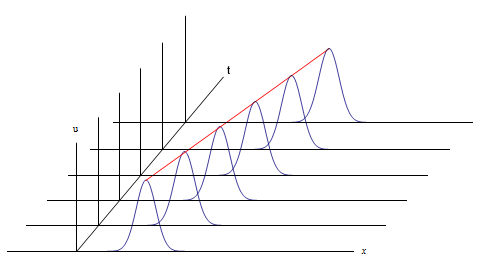
\includegraphics{Transport Equation}
\end{center}

The solution translates as time increases, which is why it's called a travelling wave solution.

In this particular case, if $x - 3t = $ constant, then $u$ is fixed.

\underline{Remarks}
%
\begin{enumerate}
  \item The parallel lines are called characteristic curves
  \item The slope of the characteristic line is $-\frac{1}{c}$ for $u_t = cu_x$.
  $c$ is the speed of the solution.
  It tells us how fast the waves are translated in the $x-$direction.
\end{enumerate}

\underline{Lemma}
%
\begin{align}
  \int^\infty_{-\infty} e^{-x^2} \text{ dx} & = \sqrt \pi
\end{align}

\begin{proof}
  Let us look at our equation squared:
  %
  \begin{align}
    I^2 & =
    \int^\infty_{-\infty} e^{-x^2} \text{ dx} \cdot
    \int^\infty_{-\infty} e^{-y^2} \text{ dy}\\
    & = \int^\infty_{-\infty} \int^\infty_{-\infty}
    e^{-x^2} \cdot e^{-y^2} \text{ dx dy}\\
    & =
    \int^\infty_{-\infty} \int^\infty_{-\infty}
    e^{-x^2 - y^2} \text{ dx dy}\\
    & =
    \int^{2 \pi}_{0} \int^\infty_0
    e^{-r^2} r \text{ dr d}\theta
  \end{align}

  Here, use polar to find our integral.
\end{proof}
\end{document}
